\synctex=1

%%%%
%%%% Multiagent Simulation and the MASON Library
%%%% Copyright 2010 by Sean Luke
%%%%
%%%% LaTeX Source
%%%% This source code, and embedded PDFs and sources (such as OmniGraffle Files)
%%%% Are distributed under the Academic Free License version 3.0
%%%% See the file "LICENSE" for more information
%%%%
%%%% When you build this source code, the resulting PDF file is licensed under the
%%%% Creative Commons Attribution-No Derivative Works 3.0 United States License
%%%% See the URL http://creativecommons.org/licenses/by-nd/3.0/us/   for more information
%%%%
%%%% If you have any questions, feel free to contact me at sean@cs.gmu.edu
%%%% Sean Luke

\documentclass[twoside,10pt]{article}
\usepackage{fullpage}
\usepackage{mathpazo}
\usepackage[noend]{algpseudocode}
\usepackage{amsmath}
\usepackage{latexsym}
\usepackage{graphicx}
\usepackage{wrapfig}
\usepackage{bm}
\usepackage{qtree}
\usepackage{array}
\usepackage{eurosym}
\usepackage{textcomp}
\usepackage{makeidx}
\usepackage{rotating}
\usepackage{multirow}
\usepackage{multicol}
\usepackage{microtype}
\usepackage{afterpage}
\usepackage{color}\definecolor{gray}{gray}{0.5}
\usepackage{alltt}
\usepackage{tabto}
\usepackage[font=footnotesize,labelsep=quad,labelfont=it]{caption}
\usepackage{todonotes}

\usepackage{listings}		% distributed 
\usepackage{xcolor}			% distributed

%%% Added in order to use hyperref -- this stuff has to appear before bibentry,x
%%% which has a conflict with regard to \bibitem.  See later in this file for more stuff that has
%%% to be added afterwards
  \makeatletter
  \let\saved@bibitem\@bibitem
  \makeatother

\usepackage{bibentry}
\usepackage[hyperfootnotes=false,linktocpage=true,linkbordercolor={0.5 0 0}]{hyperref}
%%% Note that to avoid a link being created from \pageref, just use \pageref*
%%% End hyperref stuff

\renewcommand\textfraction{0.0}
\renewcommand\topfraction{1.0}
\renewcommand\bottomfraction{1.0}


\newcommand\file[1]{\textsf{#1}}
\newcommand\variable[1]{\textsf{#1}}
%\newcommand\package[1]{\textsf{#1}}
\newcommand\package[1]{\index{Packages!{#1}}\textsf{#1}}
\newcommand\Package[1]{\index{Packages!{#1}|textbf}\textsf{#1}}
%\newcommand\class[1]{\textsf{#1}}
\newcommand\class[1]{\index{Classes!{#1}}\textsf{#1}}
\newcommand\Class[1]{\index{Classes!{#1}|textbf}\textsf{#1}}
\newcommand\method[1]{\hbox{\textsf{#1}}}
\newcommand\parameter[1]{\texttt{#1}}
\newcommand\character[1]{\texttt{"{#1}"}}
\newcommand\textstr[1]{\texttt{"{#1}"}}
\newcommand\code[1]{\textsf{#1}}

\newcommand\ignore[1]{}


\newcommand\sidebara[3]{\begin{wrapfigure}{r}[0in]{3.2in}%
\vspace{-1.1em}\hfill\framebox{\begin{minipage}{3in}\setlength\parindent{1.5em}\footnotesize{\noindent\textit{#1}

\vspace{0.5em}{\noindent #2}}
\end{minipage}}
\vspace{#3}
\end{wrapfigure}
}

\newcommand\sidebar[2]{\begin{wrapfigure}{r}[0in]{3.2in}%
\vspace{-1.1em}\hfill\framebox{\begin{minipage}{3in}\setlength\parindent{1.5em}\footnotesize{\noindent\textit{#1}

\vspace{0.5em}{\noindent #2}}
\end{minipage}}
\vspace{-0.5em}
\end{wrapfigure}
}



%%% Hack to allow more spacing before and after an hline
\newcommand\tstrut{\rule{0pt}{2.4ex}}
\newcommand\bstrut{\rule[-1.0ex]{0pt}{0pt}}

% Increase the numbering depth
\setcounter{secnumdepth}{3}
\setcounter{tocdepth}{6}


%%%% This code is used to create consistent lists of methods

% From TUGboat, Volume 24 (2003), No. 2 "Hints & Tricks"
\newcommand*{\xfill}[1][0pt]{%
	\cleaders
		\hbox to 1pt{\hss
			\raisebox{#1}{\rule{1.2pt}{0.4pt}}%
			\hss}\hfill}
			
\newenvironment{methods}[1]{
\vspace{1.0em}\noindent\textsf{\textbf{#1 Methods}}\quad \xfill[0.5ex]
\vspace{-0.25em}
\begin{description}
\small}
{\end{description}\hrule\vspace{1.5em}}

\newcommand{\mthd}[1]{\item[{\sf #1}]~\newline}


\newcommand\booktitle{MASON Discrete Event Simulation Extension}
\newcommand\reference[1]{\vspace{0.5em}\hfill{\parbox{6in}{\raggedleft\noindent\textsf{#1}}}}

% Include subsubsection in the TOC
\setcounter{tocdepth}{3}

% Use with a %, like this:   \params{%
\newcommand\params[1]{\vbox{\begin{quote}\small\tt{\noindent{#1}}\end{quote}}}
\newcommand\script[1]{\params{#1}}
\newcommand\java[1]{\params{#1}}

% Allow poor horizontal spacing
\sloppy

% Allow a ragged bottom even in two-sided
\raggedbottom

% Command to push text to following page without the cutoff that occurs with clearpage
\newcommand\bump{\vspace{10in}}

% Command to push text to following line
\newcommand\hbump{\hspace{10in}}


% Define an existing word in text as an index item
\newcommand{\idx}[1]{\index{#1}#1}

% Define an existing word in text as an index item and make it bold
\newcommand{\df}[1]{\index{#1}\textbf{#1}}

% Provide a separate index item for a word in text and make it bold
\newcommand{\dfa}[2]{\index{#1}\textbf{#2}}

% Create algorithms and definitions
\newtheorem{algm}{Algorithm}
\newtheorem{defn}{Definition}

% Initial figures, pages, algorithms, and sections should be 0 :-)
\setcounter{figure}{-1}	% Mona is Figure 0
\setcounter{page}{-1}	% Start with Page 1 (the Front Page).  I'd like it to be Page 0 but it messes up twosided
\setcounter{algm}{-1}	% Start with Algorithm 0 (the Example Algorithm)
\setcounter{section}{-1}	% Start at Section 0 (the Introduction)

\thispagestyle{plain}
\thispagestyle{empty}

\newcommand\hsp[1]{{\rule{0pt}{0pt}\hspace{#1}}}
\newcommand\spc{{\rule{0pt}{0pt}~}}


%%%% Some stuff for Distributed

\lstdefinestyle{Bash}{
  language=bash,
  basicstyle=\small\sffamily,
  numbers=left,
  numberstyle=\tiny,
  numbersep=3pt,
  frame=tb,
  breaklines=true, 
  columns=fullflexible,
  backgroundcolor=\color{yellow!20},
  linewidth=0.9\linewidth,
  xleftmargin=0.1\linewidth
}

\definecolor{javared}{rgb}{0.6,0,0} % for strings
\definecolor{javagreen}{rgb}{0.25,0.5,0.35} % comments
\definecolor{javapurple}{rgb}{0.5,0,0.35} % keywords
\definecolor{javadocblue}{rgb}{0.25,0.35,0.75} % javadoc

\lstdefinestyle{CustomJava}{
    language=java,
    basicstyle=\ttfamily,
    keywordstyle=\color{javapurple}\bfseries,
    stringstyle=\color{javared},
    commentstyle=\color{javagreen},
    morecomment=[s][\color{javadocblue}]{/**}{*/},
    numbers=left,
    numberstyle=\tiny\color{black},
    stepnumber=2,
    numbersep=10pt,
    tabsize=2,
    showspaces=false,
    breaklines=true, 
    showstringspaces=false}





\makeindex


\begin{document}

\noindent\huge\bf \booktitle\\
\\
%{\large\rm A User Manual for the MASON Multiagent Simulation Toolkit}\\
\\
\Large\bf Sean Luke\\
{\large\rm 
Department of Computer Science\\
George Mason University}
\\
\\
\\
\large\rm {\bf Manual Version 4}\\
\large\rm July 2023\\

\clearpage



\normalsize
\cleardoublepage

\tableofcontents
\clearpage

\section{Introduction}

This manual describes MASON's extension for Discrete Event Simulation (or DES).  MASON is by default an Agent-based Modeling (or ABM) toolkit, but it's relatively straightforward to build a rudimentary DES facility on top of ABM which can interoperate with it cleanly.

Many DES simulations, such as those in MASON, define a graph structure of nodes called {\it processes} which communicate by sending {\it events} to one another.  An event is the transfer of some kind of {\it resource} from one process to another.   DES simulations are particularly common for simulating supply chains, factory floors, transportation networks, and so on, where stuff moves from one fixed object to another and onward.

MASON's DES facility is built on top of its ABM facility and is designed to interoperate with it cleanly.  DES objects are placed on the Schedule (when appropriate), and they can be displayed using MASON's standard displays and portrayals.  Furthermore, there's nothing stopping agents from interacting with DES processes or resources.  If you've wanted to build a hybrid ABM and DES tool, now is your chance!

This manual assumes you're pretty familiar with MASON.  It assumes you know what SimState and Schedule are, how to schedule objects, how to create a SimState subclass, how to create a GUIState, how to build Displays and Field Portrayals, and so on.  If you're not familiar with this stuff, it's time to peruse the MASON manual and perhaps build some standard MASON demo examples.

The DES extension is entirely contained within the directory \file{sim}, located in the \file{contrib/des} directory.  You can build a jar file of this directory as:
\\
\\
\code{cd contrib/des}\\
\code{javac sim/*.java sim/*/*.java sim/*/*/*.java sim/*/*/*/*.java}\\
\code{jar -cvf des.jar sim/}
\\

... and then add \code{des.jar} to your development library.

\begin{figure}[t]
\centering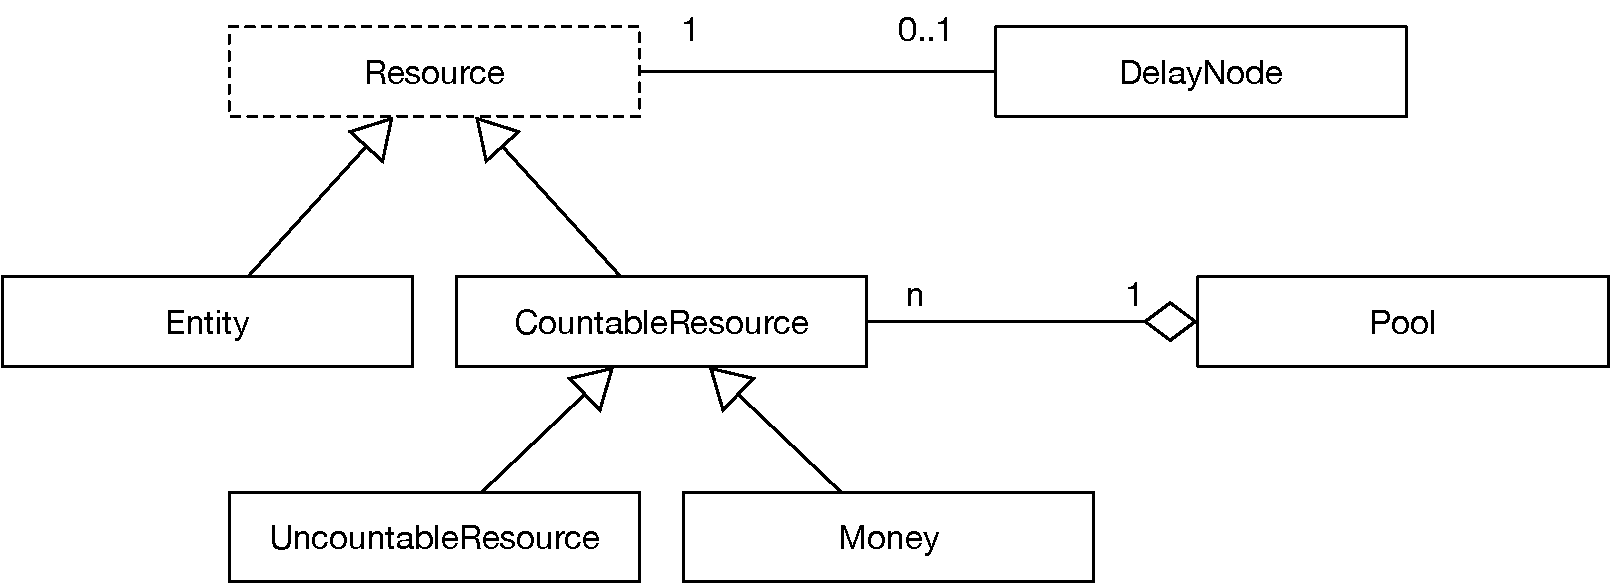
\includegraphics[width=4in]{Resources.pdf}
\end{figure}

\subsection{Class Overview}

MASON's DES classes may be roughly divided into four categories: {\bf Resources}, {\bf Processes}, {\bf Composed Processes}, and {\bf Visualization Tools}.  Processes communicate with one another by giving each other Resources.  The whole model is visualized using the visualization tools.

\paragraph{Resources}  Money, love, gasoline, palettes of goods, cargo containers, water, and people waiting in line are all resources.  They're things handed off from process to process to make a DES simulation hum.  The abstract superclass is {\bf Resource}.   A simple Resource is {\bf Entity}, an atomic object like a skeeball ticket or a video game token.  Entities can also serve as containers for collections of Resources, much like a cargo container, a truck of goods, or a palette of microwaves.  
these are called  {\it Eomposite Entities}.  {\bf CountableResources} are Resources which can have have integer amounts greater than one (they're not Entities) and cannot be infinitely subdivided.  For example, you can have 1000 medicine pills, or 200 eggs, but you can't have half an egg.  {\bf Money} is a CountableResource which prints nicely (like \$4.32).  {\bf UncountableResources} are Resources which are infinitely subdivisible, like water or love or gasoline or time.  You can make as many Resources as you like of various types, as members of these general classes.

\paragraph{Processes}  A Process is an object which hands resources to another process or receives the same.  There are three major abstract kinds of Processes.  A {\bf Provider} provides resources.  A {\bf Receiver} receives resources from a Provider.  A {\bf Middleman} is both a Provider and a Receiver: it receives resources from Providers, and then provides them to downstream Receivers.

MASON's DES system is mostly a ``push'' system: providers generally offer resources to receivers (who may choose to accept or reject the offer).  However in many cases it also has an optional ``pull'':  receivers can ask providers offer resources to them (or in some cases, to offer resources to {\it other} receivers), and providers may respond to these entreaties or ignore them.

Consider a classic MM1 Queue: people arrive at a bank, then waiting in line at a bank teller.  Here people are represented as Entities.  They are generated by a {\bf Source}, which produces the people entering the bank.  Sources can produce resources (people) at random, via a schedule, and so on.  The Source then hands its produced people to a {\bf Queue}, which represents the line they have to wait in.  A Queue can also be thought of as a warehouse of items waiting to be processed.  The Queue then attempts to feed people through a {\bf Lock}, which only allows people to pass if it can allocated a different Resource (let's call it a Teller) from a {\bf Pool} of Tellers.  In our case there's only a single Teller, so if the Pool doesn't have one available for the Lock, the Lock refuses to let the next person move forward.  when a Lock can allocate a Teller and let a person move forward, the person is handed off to a {\bf SimpleDelay}, which holds the person for a fixed amount of time, representing the time the Teller needs to service the person.  When the SimpleDelay lets go of the person, it is handed off to an {\bf Unlock}, which places the Teller resource back in the Queue and informs the Lock that a Teller is available again.  The person is then finally handed to a {\bf Sink}, which is basically a black hole in which Resources disappear forever, and represents the end of the line for people in the model.

There are actually three kinds of Delays available.  A SimpleDelay delays resources for a fixed amount of time.  A Delay delays them for a varying amounts of time (but is more costly).  A BoundedDelay delays them for varying amounts of time as long as those times are integer values less than some number \(N\) (it's cheaper than a Delay).

Some more processes.  An {\bf If} receives incoming Resources and sends them to one or another of different downstream receivers based on some decision you specify.  A {\bf Composer} takes multiple different resources and packs them together into a Composite Entity.  A {\bf Decomposer} does the opposite.  An {\bf Extractor} is a kind of Source which produces resources by requesting them from another Provider.  A {\bf Transformer} is like a currency converter: it accepts Resources and produces (converts them into) different kinds of Resources.  A {\bf Probe} lets Resources pass through it, but records the amount and rate for statistical purposes.  It can be used in combination with a {\bf Lead}: together they can measure the amount and rate of Resource passing through a subgraph of processes.

These Processes are all designed to be subclassed and customized to your heart's content.

\paragraph{Composed Processes}

MASON provides two ways to compose Processes.  First, there are {\bf Macros}.  A Macro wraps a subgraph of Processes in a neat little package and lets you repeat this subgraph over and over cleanly.  It's a useful abstraction tool.  A {\bf Service} is a commonly used Macro.  

Second, there are {\bf Multis}.  Normally Processes deal with one incoming type of Resource and one outgoing type of Resource, often the same.  But a Multi lets you have many incoming and outgoing types of Resources from different sources and destinations. You might use a Multi to model a bicycle factory: it takes steel, and bike components, and energy, and produces bicycles and trash.  Muiltis are meant to be customized: they don't do anything interesting on their own.

\paragraph{Visualization Facilities}

All of the DES system's processes, and their interconnections may be visualized and inspected using standard MASON facilities.  To make this easy, the processes serve as their own Simple Portrayals, and DES system provides a variety of tools to display them and customize them.
  
\section{Resources and Related Objects}

The MASON DES extension largely consists of two basic kinds of classes:  {\bf Resources} and {\bf Processes}, plus visualization tools of the same.   Processes perform actions in response to events.  In most cases, this action involves Processes handing off Resources to other Processes.  This could be for many reasons.  Perhaps a Resource moving from Process A to Process B to another represents A paying B for some service.  Perhaps Processes A and B are warehouses and the Resource represents a truck moving from one to the other.  Perhaps A and B are countries and the Resource represents a family migrating.  Maybe A and B are spies and the Resource holds a critical communication between them.

Resources are also held in {\bf Pools}.  A Pool can be dipped into by certain Processes to allocate a Resource for some temporary function.  For example, imagine if a factory floor had four assembly lines but only two lathes.  Widgets moving through an assembly line at some point had to be lathed, and if a lathe was not available, the widget (and its assembly line) would have to wait until one came available.

To do this, there are two special kinds of Processes, copies of which are part of each assembly line, called {\bf Lock} and {\bf Unlock}.  For a widget to pass through a Lock, the Lock must first allocate a Resource (representing the lathe) from a shared Pool.  If it cannot, the widget must wait until the Lock can allocate the Resource.  Then the widget may pass through to other Processes.  Ultimately when widget is finished with the lathe, the widget can pass through an {\bf Unlock} Process, which gives a Resource back to the Pool.   The Pool only holds two lathe Resources.\footnote{These are called Lock and Unlock because they are reminiscent of locking or unlocking on a mutex or a semaphore in computer science terminology.   So sue me, I'm a computer science professor. Others in the Discrete Event Simulation world might instead refer to {\bf seizing} and {\bf releasing} resources from a pool.}

Resources are often passed through {\bf Delays}, Processes which hold them up for a certain amount of time.  To manage this time, Delays will store Resources in {\bf DelayNodes} and associate them with timestamps. 
  
MASON provides several kinds of Resources, depending on your modeling needs:

\begin{itemize}
\item {\bf Entities} are atomic elements, like tickets or tokens or cars.  They cannot be broken up into smaller Entities, nor joined together to form larger ones.  They are not worth different amounts: an Entity is an Entity.
\item {\bf Composite Entities} are Entities which hold a collection of other Resources inside them, plus a manifest.  For example, a Composite Entity might be used to model a shipping container filled with teddy bears.  The manifest can indicate anything you'd like: expiration dates, country of origin, who manufactured each teddy bear, the amount of love that went into each teddy bear, and so on.  There is a special Process called a {\bf Composer} which takes a collection of Resources and builds a Composite Entity 
\item {\bf Countable Resources} are Resources which can be divided, but only as integers.  For example, packages of medicine pills are countable resources: the package could be 0 pills, or 1 pill, or 2 pills, or 1500 pills.  But it cannot be 1.5 pills.  You cannot have a negative or infinite value.
\item {\bf Money} is an obvious example of a Countable Resource.  In US currency, the fundamental unit of money is the penny.  You cannot have a half a penny, and you cannot have 3.279 pennies.\footnote{Except on the stock exchange.}  Because money is so common, MASON has a dedicated kind of Countable Resource just to represent it: it prints it out in a pleasing fashion (like ``\$14.23'' for 1423 pennies). 
\item {\bf Uncountable Resources} are Resources which can be divided indefinitely.  An example of an uncountable resource is water.  You can have 3.239122 liters of water, and you can divide that into five parts any way you like, including some parts holding 0 liters.  You cannot have a negative or infinite value.
\end{itemize}

Resources are typed, and you can have as many different types of Resources as you like.  For example, you could have a type of Countable Resource representing pills and another one representing punches in the face.  You could have a type of Uncountable Resource representing water and another one representing love.  You could have both US dollars and Hong Kong dollars.  You could have both cargo containers and suitcases of stuff.  These types are not exchangeable: you can't give a Process water when it's expecting love.  However there exists a special Process, called a {\bf Transformer} which can convert certain Resources into Countable Resources: for example, it could be used as a currency converter.     

If Resources are typed, how do you make a new type of Resource, and how do you make more of that same type?  Each Resource type has a unique name.  To make a new type of resource, just instantiate a Resource class with that new name.  Later Resources of that type are allocated by copying them from earlier Resources of the same type. This can be done either by calling \method{duplicate()} or by calling a copy constructor on the earlier Resource, indicating the amount of the new Resource.

Processes deal with Resources differently based on the kind of Resources.  For example, many Processes store Resources to eventually hand off to downstream Processes.  If the Resource is an Entity, then it is atomic and the Process must store it in a collection of Entities.  If the Resource is a Countable or Uncountable Resource, then the Process can simply merge it into one pile or blob of Countable (or Uncountable) Resource, and dole it out as appropriate later on.

All Resources have {\bf amounts}.  For Countable or Uncountable resources, the amount is simply the size of the resource: such as 1500 pills or 1423 pennies or 3.239122 liters of water.  For Entities, including Composite Entities, the amount is always 1.

\subsection{Resource}

Resource is the abstract superclass of all resources.  All Resources have a {\bf unique type} (an integer) shared by resources of that type, and a {\bf name} (a String) which you can stipulate.  For example, all Electricity resources might have type 0, and all Gas resources might have type 1 and all Cars might have type 2 and all Dollars might have type 3.  It is possible to construct two Resources with the same name, but they will have different types even so: don't do that.  For your own sanity, make sure that you only construct a Resource once with a given name, and copy Resources from it to make more of the same type.

\begin{methods}{\class{sim.des.Resource} Constructor}
\mthd{public Resource(String name)}
Builds a new Resource, of a new unique type, with the given name.
\mthd{protected Resource()}
Builds a new Resource, but does not set the name or type.  This exists to permit copy constructors in subclasses.  Normally you'd leave it alone.
\end{methods}

\begin{methods}{\class{sim.des.Resource}}
\mthd{public void clear()}
Clears the resource. What this does varies depending on the subclass.
\mthd{public void toString()}
Prints the resource in a pleasing manner.
\mthd{public boolean equals(Object other)}
Returns true if {\it other} is exactly the same object as this Resource.  This is a comparison by pointer rather than by value, because Resources are generally mutable. 
\mthd{public int hashCode()}
Returns an appropriate hash code for hash tables.
\mthd{public double getAmount()}
Returns the amount of the Resource.  Note that this is always double, even for Countable Resources and for Entities, both of which return integers.
\mthd{public boolean isSameType(Resource other)}
Returns true if {\it other} is not null and the same type as this Resource. 
\mthd{public int getType()}
Returns the type of this resource. 
\mthd{public String getName()}
Returns the name of this resource. 
\mthd{protected void setName(String name)}
Sets the name of this resource.  You shouldn't call this probably.
\mthd{public Resource duplicate()}
Exactly duplicates the Resource once and returns the result.  The storage and info objects are not copied\,---\,just pointer-copies.  You'll have to deep copy them as you see fit.
\mthd{public Resource[] duplicate(int times)}
Exactly duplicates the Resource {\it times} times and returns the result.  The storage and info objects are not copied\,---\,just pointer-copies.  You'll have to deep copy them as you see fit.
\end{methods}


\subsection{Entity}

An Entity is a Resource that cannot be subdivided into smaller Resources of the same time.  For example: a Car might be an Entity.  But Water is not, as you can divide Water up into smaller amounts.  Entities can {\bf store} other resources inside them: that is, they can be {\bf composed} of them.  For example, a given Car might contain Wheels, and Engine, and some amount of Gasoline.  Different Cars are permitted to store different things.  Entities can also contain {\bf info} objects, essentially manifests.

\begin{methods}{\class{sim.des.Entity} Constructor}
\mthd{public Entity(String name)}
Builds a new Entity, of a new unique type, with the given name.
\mthd{public Entity(Entity other)}
Makes a copy of the Entity, including its type and name.  The storage and info objects are pointer-copied, not deep-copied.  This is the standard copy constructor for Entity.
\end{methods}

Here are the custom methods for Entity.  It also implements the methods defined in Resource.

\begin{methods}{\class{sim.des.Entity}}
\mthd{public Resource[] getStorage()}
Returns the actual storage array of the Entity, or null if there isn't one.
\mthd{public void setStorage(Resource[] val)}
Sets the storage array of the Entity.  This can be set to null.
\mthd{public Object getInfo()}
Returns the actual info object of the Entity, or null if there isn't one.
\mthd{public void setInfo(Object val)}
Sets the info object of the Entity.  This can be set to null.
\mthd{public boolean isComposite()}
Returns true if the storage is non-null.
\mthd{public void clear()}
Sets the storage to null.
\mthd{public double getAmount()}
Always returns 1.0.
\end{methods}

\subsection{CountableResource}

A CountableResource is a Resource that has an {\bf amount} (an integer) and can be subdivided into CountableResources with smaller integer amounts.  For example: a Population might be divided into smaller subpopulations.  There is an atomic, smallest, non-divisible amount of CountableResources: 1.  You can also set the amount to 0.

Even though CountableResource only stores integers for amounts, it stores them as doubles.  This means that its maximum integer value is larger than that of an int.  Specifically, it is equal to \variable{sim.des.CountableResource.MAXIMUM\_INTEGER}

\begin{methods}{\class{sim.des.CountableResource} Constructor}
\mthd{public CountableResource(String name, double intialAmount)}
Builds a new CountableResource, of a new unique type, with the given name and amount.
\mthd{public CountableResource(String name)}
Builds a new CountableResource, of a new unique type, with the given name and zero amount.
\mthd{public CountableResource(CountableResource other)}
Makes a copy of the CountableResource, including its type, name, and amount.  If the provided object is actually an UncountableResource, this will throw an exception.
\mthd{public CountableResource(CountableResource other, double initialAmount)}
Makes a copy of the CountableResource, including its type and name, but with the new amount provided.    If the provided object is actually an UncountableResource, this will throw an exception.
\end{methods}

Here are the custom methods for CountableResource.  It also implements the methods defined in Resource.

\begin{methods}{\class{sim.des.CountableResource}}
\mthd{public double doubleValue()}
Returns the amount as a double value.
\mthd{public boolean isUncountable()}
Returns false (note that this is overridden by UncountableResource).
\mthd{public boolean isCountable()}
Returns true (note that this is overridden by UncountableResource).
\mthd{public double getAmount()}
Returns the amount stored in the CountableResource, which will always be a nonnegative integer (but possibly larger than an int).
\mthd{public void clear()}
Sets the amount to 0.
\mthd{public double getAmount()}
Returns the amount.
\mthd{public void setAmount(double val)}
Sets the amount
\mthd{public void bound(double min, double max)}
Bounds the resource to be no more than max and no less than min.  It must be the case that max \(\geq\) min \(\geq\) 0.
\mthd{public void bound(double max)}
Bounds the resource to be no more than max and no less than zero.  It must be the case that max \(\geq\) 0.
\mthd{public boolean increase(double val)}
Increases the amount by the given value and returns true, unless val is not an integer, or unless this would exceed \variable{sim.des.CountableResource.MAXIMUM\_INTEGER}, in which case nothing happens and false is returned.
\mthd{public boolean decrease(double val)}
Decrements the amount by the given value and returns true, unless val is not an integer, or unless this would drop below zero, in which case nothing happens and false is returned.
\mthd{public boolean increment()}
Increments the amount by 1 and returns true, unless this would exceed \variable{sim.des.CountableResource.MAXIMUM\_INTEGER}, in which case nothing happens and false is returned.
\mthd{public boolean decrement()}
Decrements the amount by 1 and returns true, unless this would drop below zero, in which case nothing happens and false is returned.
\mthd{public CountableResource reduce(double atLeast, double atMost)}
Subtracts at least a certain amount and at most a certain amount from this CountableResource, placing that amount into a new CountableResource and returning it, unless there is not enough amount to do so, in which case nothing happens and false is returned.  atLeast and atMost must be integers, with atMost \(\geq\) atLeast \(\geq\) 0.
\mthd{public CountableResource reduce(double byExactly)}
Subtracts exactly a certain amount from this CountableResource, placing that amount into a new CountableResource and returning it, unless there is not enough amount to do so, in which case nothing happens and false is returned.  byExactly must be an integer \(\geq\) 0.
\mthd{public void add(CountableResource other)}
Adds the other CountableResource's amount into this one, setting the other CountableResource's amount to zero afterwards.
\mthd{public void add(CountableResource other, double atMostThisMuch)}
Adds atMostThisMuch of the other CountableResource's amount into this one, setting the other CountableResource's amount to the remainder afterwards.
\mthd{public void add(CountableResource[] other)}
Adds all the other CountableResources' amounts into this one, setting the other CountableResources' amounts to zero afterwards.
\mthd{public boolean greaterThan(CountableResource other)}
Returns true if this amount is greater than the other resource's amount.
\mthd{public boolean greaterThanOrEqualTo(CountableResource other)}
Returns true if this amount is greater than or equal to the other resource's amount.
\mthd{public boolean lessThan(CountableResource other)}
Returns true if this amount is less than the other resource's amount.
\mthd{public boolean lessThanOrEqualTo(CountableResource other)}
Returns true if this amount is less than or equal to the other resource's amount.
\mthd{public boolean equalTo(CountableResource other)}
Returns true if this amount is equal to the other resource's amount.  Compare to equals(...), which is only true if the two objects are literally the same, by pointer.
\mthd{public int compareTo(Object other)}
Returns 0 if the other object's amount is equal to, -1 if it is greater than, and 1 if it is less than my amount.   Note that though this is not a requirement of the compareTo(...) contract, compareTo(...) here is not consistent with equals(...), which does pointer comparison.
\end{methods}



\subsection{Money}

Money is a CountableResource with a cute printing function which prints it with a currency sign.  For example, a Dollar is Money, hence a CountableResource, where the smallest amount (1) would be the Cent.  Perhaps it should be renamed Cents.

\begin{methods}{\class{sim.des.Money} Constructor}
\mthd{public Money(String name, double intialAmount)}
Builds a new Money, of a new unique type, with the given name and amount.  The name will be used as a currency symbol during printing.
\mthd{public Money(String name)}
Builds a new Money, of a new unique type, with the given name and zero amount.   The name will be used as a currency symbol during printing.
\mthd{public Money(Money other)}
Makes a copy of the Money, including its type, name, and amount.
\mthd{public Money(Money other, double intialAmount)}
Makes a copy of the Money, including its type and name, but with the new amount provided.
\end{methods}

Here are the custom methods for Money.  It also implements the methods defined in CountableResource.

\begin{methods}{\class{sim.des.Money}}
\mthd{public String toString()}
Returns the amount in decimal format as \(CX.Y\), where \(C\) is the name (a currency symbol), \(X\) is the amount / 100, and \(Y\) is the amount mod 100.  For example, if ``\$'' was the name, and the amount was 1423, then this would print as ``\$14.23''
\end{methods}


\subsection{UncountableResource}

An UncountableResource is a CountableResource which can be subdivided infinitely and has real-valued amounts.  Thus while you can only have a CountableResource with values 0, 1, 2, 3, ...., an UncountableResource could be any positive amount, such as 0 or 2.34129 or 92.3 or Infinity.

If you have a variable holding a CountableResource, how do you know it is a CountableResource versus an UncountableResource?  You could use {\tt instanceof}, or you could call {\tt isCountable()} or {\tt isUncountable()}.

\begin{methods}{\class{sim.des.UncountableResource} Constructor}
\mthd{public UncountableResource(String name, double intialAmount)}
Builds a new UncountableResource, of a new unique type, with the given name and amount.
\mthd{public UncountableResource(String name)}
Builds a new UncountableResource, of a new unique type, with the given name and zero amount.
\mthd{public UncountableResource(UncountableResource other)}
Makes a copy of the UncountableResource, including its type, name, and amount.
\mthd{public UncountableResource(UncountableResource other, double intialAmount)}
Makes a copy of the UncountableResource, including its type and name, but with the new amount provided.
\end{methods}

Here are the custom methods for UncountableResource.  It also implements the myriad of methods defined in CountableResource.

\begin{methods}{\class{sim.des.UncountableResource}}
\mthd{public UncountableResource[] divide(int times)}
Divides the amount by {\it times}, which must be \(> 0\), and builds {\it times} \(-1\) new UncountableResources, each with the new amount.  Also reduces the amount of this UncountableResource to the amount as well. 
\mthd{public UncountableResource halve()}
Builds a new UncountableResources with half the amount, leaving the other half as the current amount.
\mthd{public void scale(double value)}
Changes the amount by multiplying it by the given value.
\mthd{public boolean increase(double val)}
Increases the amount by the given value and returns true.
\mthd{public boolean decrease(double val)}
Decrements the amount by the given value and returns true, unless this would drop below zero, in which case nothing happens and false is returned.
\end{methods}




\subsection{Pool}

A {\bf Pool} is a storage of a single kind of CountableResource, UncountableResource, or Money.   Various Process objects, namely {\bf Lock} and {\bf Unlock}, dip into a shared Pool to add or remove resources or to wait until resources have come available.

Pool is very simple: it has a {\bf maximum} amount of resource, a {\bf minimum} (always zero), and an {\bf initial resource allocation}.   Beyond that, its current resource can be set and queried.  And that's it!

A Pool extends \class{sim.des.portrayal.DESPortrayal}, so it can serve as a MASON SimplePortrayal.  DESPortrayal objects are also \class{sim.des.Named}, so the Pool can be given a name via \method{getName()} and \method{setName(...)}.

A Pool is \class{sim.des.Resettable}, meaning that it can be reset to its original state via a method called \method{reset(...)}.


\begin{methods}{\class{sim.des.Pool} Constructor}
\mthd{public Pool(CountableResource resource, double maximum)}
Builds a Pool of the given type of CountableResource, with an initial amount copied from the CountableResource, and the provided maximum.
\mthd{public Pool(CountableResource resource)}
Builds a Pool of the given type of CountableResource, with an initial amount copied from the CountableResource, and a maximum of infinity (if it's an UncountableResource), or \variable{CountableResource.MAXIMUM\_INTEGER} (if it's a CountableResource or Money).
\mthd{public Pool(double initialResourceAllocation)}
Builds a Pool of a new type of CountableResource, with an initial amount as specified, and a maximum of infinity (if it's an UncountableResource), or \variable{CountableResource.MAXIMUM\_INTEGER} (if it's a CountableResource or Money).
\mthd{public Pool(double initialResourceAllocation, double maximum)}
Builds a Pool of a new type of CountableResource, with an initial amount as specified, and the specified maximum.
\end{methods}

A Pool only has a few methods:

\begin{methods}{\class{sim.des.Pool}}
\mthd{public void reset(SimState state)}
Resets the Pool.   This simply resets its current amount to the initial amount: the name and maximum stay as you had last set them.
\mthd{public CountableResource getResource()}
Returns the current available resource.
\mthd{public void setResource(CountableResource val)}
Sets the current available resource.
\mthd{public double getMaximum()}
Returns the maximum allowed resource.
\mthd{public void setMaximum(double value)}
Sets the maximum allowed resource.
\mthd{public String getName()}
Returns the name (which can be null).
\mthd{public void getName(String name)}
Sets the name (which can be null).
\mthd{public String toString()}
Returns the Pool and its state in a pleasing fashion.
\end{methods}



\subsection{DelayNode}

A {\bf DelayNode} holds a Resource and associates it with a timestamp and a {\bf Provider} (a Process which provided the Resource, discussed later).  DelayNodes can be strung together into small Linked Lists.    DelayNodes are used by various delays (SimpleDelay, Delay, and BoundedDelay) to describe how long a Resource must be delayed before the delay Process makes it available to others.  Additionally, a DelayNode can be marked {\bf dead}, meaning that its Resource has been destroyed and will no longer be available to others after it leaves the delay. 

\begin{methods}{\class{sim.des.DelayNode} Constructor}
\mthd{public DelayNode(Resource resource, double timestamp, Provider provider)}
Builds a DelayNode with the given resource, timestamp, and provider.
\end{methods}

\begin{methods}{\class{sim.des.Delay}}
\mthd{public Resource getResource()}
Returns the resource.
\mthd{public double getTimestamp()}
Returns the timestamp.
\mthd{public Provider getProvider()}
Returns the provider.
\mthd{public boolean isDead()}
Returns whether the Resource has been marked dead.
\mthd{public void setDead(boolean val)}
Marks the Resource as dead.
\end{methods}


\clearpage
\begin{figure}[t]
\centering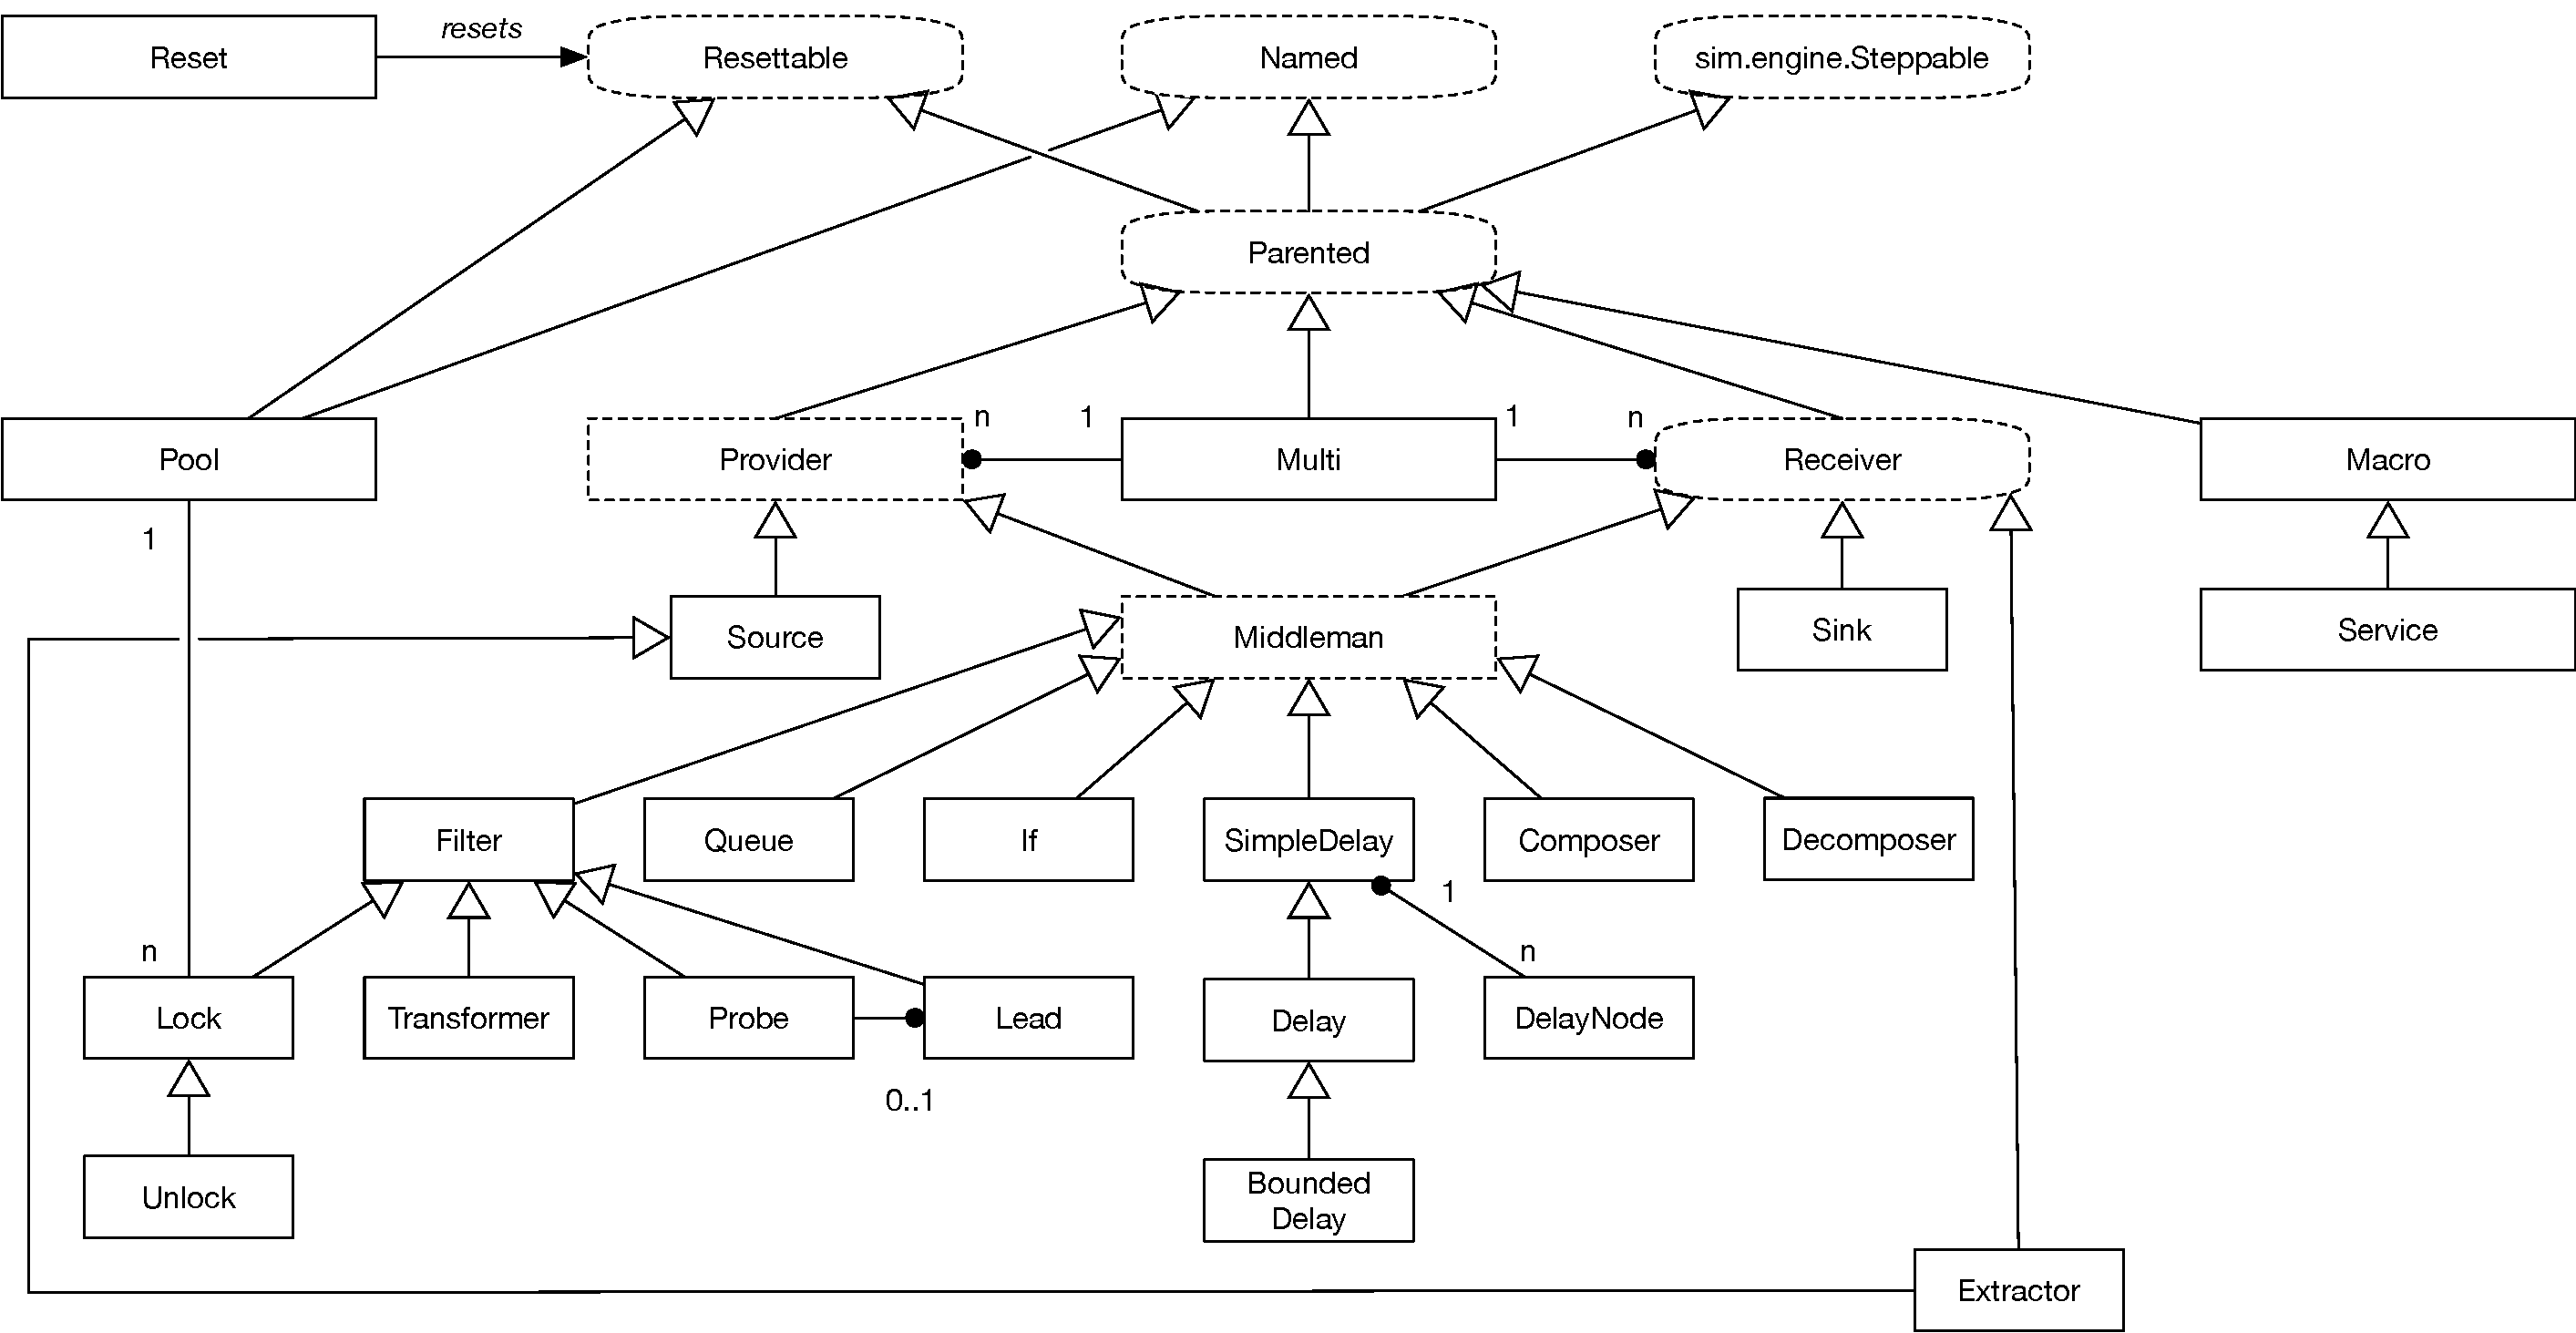
\includegraphics[width=6.5in]{Processes.pdf}
\end{figure}

\section{About Processes}

Processes are the verbs of the DES system.  They perform actions in response to {\it events} (or if you like, {\it signals}) they receive.  

An event can be one of four things typically:

\begin{itemize}
\item Another Process can {\it offer} some Resources to the Process, asking it to {\it accept} them.
\item Another Process can {\it request} that the Process offer (or {\it provide}) it a resource.
\item Another Process can {\it offer a transaction} (an exchange) of a Resource for some other Resource.
\item MASON's Schedule can wake up the Process and tell it to do some work.
\end{itemize}

Only certain Processes do certain kinds of events.  The various Process objects can be {\bf Receivers} or {\bf Providers}, or they can be both (known as a {\bf Middleman}).  A special subclass of Middleman, called a {\bf Filter}, is designed to pass received resources from Providers directly to downstream Receivers in zero time.    Subgraphs of Process objects can be packed into a single object called a {\bf Macro}.    

Indeed most Process objects do their work in zero time, the notable exception being various kinds of {\bf Delays}.

Most Process objects are meant to receive and/or provide a resource of a single type.  If you need a Process which works with several types of Resources, you can  use a {\bf Multi}, which provides several Receivers and Provides that work in concert.  For example, you might use a Multi to represent a factory which takes steel, labor, and electricity and produces bicycles and waste (five different Resource types).

Process objects inherit from a variety of high-level abstract classes and interfaces, so let's start there.

\section{Abstract Process Superclasses and Interfaces}

\subsection{Resettable and Reset}

All Processes are Resettable, meaning they can be {\bf reset}.  A convenience Reset object is provided which can reset multiple Resettable objects at once.

\begin{methods}{\class{sim.des.Resettable}}
\mthd{public void reset(SimState state)}
Resets the object to its initial state.
\end{methods}

\begin{methods}{\class{sim.des.Reset} Constructor}
\mthd{public Reset(SimState state)}
Constructs a Reset object.
\end{methods}

\begin{methods}{\class{sim.des.Reset}}
\mthd{public void reset()}
Resets all the objects stored in the Reset.
\mthd{public void add(Resettable r)}
Stores an object in the Reset.
\mthd{public void remove(Resettable r)}
Removes an object from the Reset.
\end{methods}

\subsection{Named}

All Processes are Named, meaning that they have a {\bf name} (a String).

\begin{methods}{\class{sim.des.Named}}
\mthd{public String getName()}
Returns the name, or null.
\mthd{public void setName(String name)}
Sets the name.
\end{methods}

\subsection{sim.engine.Steppable}

A Steppable is an object which can be placed on MASON's schedule to be stepped in the future.  All processes are Steppable, but only a few need it. [Perhaps in the future we may be more selective in this regard].

\begin{methods}{\class{sim.engine.Steppable}}
\mthd{public void step(SimState state)}
Steps the Steppable to do work.
\end{methods}

\subsection{Parented}

Processes are Parented, meaning that they have a parent who ``owns'' the Process and will take care of it, stepping it and resetting it as necessary.   All Parented objects are Resettable, Named, and sim.engine.Steppable.  

\begin{methods}{\class{sim.des.Parented}}
\mthd{public Object getParent()}
Returns the parent, or null if no parent.
\mthd{public void setParent(Object parent)}
Sets the parent.  Pass in null to remove the parent.
\end{methods}

\subsection{Receiver}

An object which can {\it receive} an offer from a Provider.  That is, the Provider will offer the Receiver some amount of Resource, asking it to {\bf accept} the offer.  Offers have minimum and maximum amounts that the Receiver may select from.  The receiver accepts some appropriate amount (between the min and max) of the Resource being offered by the Provider, or it refuses it.  A Receiver can also go to a Provider and {\bf ask} that the Provider make an offer to the Receiver.  Receivers have a {\bf typical Resource type} of the resource that they accept.  Rarely, a Receiver can receive more than one resource.

\begin{methods}{\class{sim.des.Receiver}}


\mthd{public Resource getTypicalReceived()}
Each Receiver is designed to receive a certain type of Resource called the {\it typical} Resource.  This method returns a Resource of this type for type comparison purposes.

\mthd{public void setRefusesOffers(boolean value)}
Sets whether this Receiver should unilaterally refuse all offers.

\mthd{public boolean getRefusesOffers()}
Returns whether this Receiver is presently unilaterally refusing all offers (that is, setRefusesOffers(...) was turned on).

\mthd{public boolean accept(Provider provider, Resource resource, double atLeast, double atMost)}
This method is called to ask the Receiver to {\bf accept an offer} of some amount of a given resource from a given provider.   If the Receiver accepts some of the resource, it returns true, else it returns false if it refuses the resource.   This method may throw a RuntimeException if the resource does not match the typical resource of the receiver, or if a cycle was detected in accepting offers (A offers to B, which offers to C, which then offers to A).  It should be the case that \(0 \leq\) {\it atLeast} \(\leq\) {\it atMost} \(\leq\) resource.getAmount(), else a RuntimeException will be thrown.  Though atLeast may be set to 0, Receivers must never accept 0 of any resource: they must always accept more than 0, or else refuse.  If the Receiver is currently refusing all offers, this method should always return false.

If the Resource is an Entity, the Receiver takes control of the entire Resource.  {\it atLeast} and {\it atMost} may be ignored (and in general should be set to 0 and 1 respectively).

If the Receiver is a CountableResource (or an UncountableResource or Money etc.), then the Receiver may remove between {\it atLeast} and {\it atMost} (inclusive) amount of the provided Resource.

it returns true, else it returns false if it refuses the resource.   If the Resource is an Entity, the Receiver takes control of the entire Resource.  {\it atLeast and atMost} may be ignored (and in general should be set to 0 and 1 respectively).

\end{methods}

\subsection{Provider}

An object which can make offers to one or more Receivers.  Receivers are {\bf registered} with the Provider.  When the Provider has a resource to offer, it will go to each of its Receivers according to some {\bf offer policy} and ask them to {\bf accept} offers of the Resource until it is depleted.  Providers can also be asked by a Receiver to make an offer to it.    Providers have a {\bf typical Resource type} of the resource that they offer.  Rarely, a Provider can provide more than one resource.

\begin{methods}{\class{sim.des.Provider} Constructor}
\mthd{public Provider(SimState state, Resource typicalProvided)}
Constructs a Provider object given the provided SimState and typical provided resource.
\end{methods}

\begin{methods}{\class{sim.des.Provider}}
\mthd{public SimState getState()}
Returns the SimState model object.

\mthd{public Resource getTypicalProvided()}
Each Provider is designed to provide a certain type of Resource called its {\it typical} Resource.  This method returns a Resource of this type for type comparison purposes.
\end{methods}


\paragraph{Storing Resources}
A Provider maintains a pool of resources to offer to downstream Receivers.    This pool can be one of two types: either a single collected Resource, or an ordered list of available Entities.  Accordingly Providers have two {\bf protected} variables:

\begin{itemize}
\item {\tt protected CountableResource resource;}
\item {\tt protected LinkedList\(<\)Entity\(>\) entities;}
\end{itemize}

One of these will be \variable{null}.  This is determined by the typical provided Resource type of the Provider.  If the type is a subclass of CountableResource, then \variable{entities} will be nulled out.  If the type is a subclass of Entity, then \variable{resource} will be nulled out.  Subclasses of Provider are free to add or remove from the non-null variable: but you should not change which one is null and which is non-null.

\begin{methods}{\class{sim.des.Provider}}
\mthd{public SimState clear()}
Clears the stored resources.

\mthd{public double getAvailable()}
Returns the total amount of stored resources.  If the resources are CountableResources, this returns \variable{resource.getAvailable()}  If the resources are Entities, this returns \variable{entities.size()}

\mthd{public Entity[] getEntities()}
Returns in an array all the current Entities the Provider can provide.  You can
        modify the array (it's yours), but do not modify the Entities stored inside, as they
        are the actual Entities stored in the Provider.  If this Provider does not provide
        Entities, then null is returned.  

\mthd{public Entity getEntity(int entityNumber)}

       Returns the available entity with the given number for inspection, but does not remove it from the available pool.
       Numbers range from 0 to (int)getAvailable();  You probably should not modify this Entity: it is the actual
       Entity in the Provider and is owned by the Provider.  If this Provider does not offer entities, or if
       the entityNumber is invalid, an exception is thrown.

\end{methods}

\paragraph{Registering Receivers}
A Provider maintains a list of Receivers who have registered themselves to receive offers from it.  Note that Receivers do not maintain a corresponding list of Providers.

\begin{methods}{\class{sim.des.Provider}}
\mthd{public boolean addReceiver(Receiver receiver)}
Registers a Receiver.  Receivers may not be registered multiply with the same Provider.  Returns false if the Receiver had already been registered with this Provider.
\mthd{public boolean removeReceiver(Receiver receiver)}
Deregisters and removes a Receiver.  Returns false if the Receiver was not registered.
\mthd{public ArrayList\(<\)Receiver\(>\) getReceivers()}
Returns all registered receivers.  
\end{methods}

\paragraph{Making Offers}  This is what Providers do: they make offers to Receivers.  To do this, a Provider subclass would call offerReceivers() or [rarely] offerReceivers(...).  Then the Provider will offer resources to its Receivers according to its {\bf offer policy} and {\bf offer order}.

The offer policy governs the way and order in which offers are made to Receivers.  The options are:

\begin{verbatim}
    /** Offer Policy: offers are made to the first receiver, then the second, and so on, 
         until available resources or receivers are exhausted. */
    public static final int OFFER_POLICY_FORWARD = 0;
    
    /** Offer Policy: offers are made to the last receiver, then the second to last, 
         and so on, until available resources or receivers are exhausted. */
    public static final int OFFER_POLICY_BACKWARD = 1;
    
    /** Offer Policy: offers are made to the least recent receiver, then next, and so on, 
         until available resources or receivers are exhausted. */
    public static final int OFFER_POLICY_ROUND_ROBIN = 2;
    
    /** Offer Policy: offers are made to the receivers in a randomly shuffled order, 
         until available resources or receivers are exhausted. */
    public static final int OFFER_POLICY_SHUFFLE = 3;
    
    /** Offer Policy: offers are made to only one random receiver, chosen via an 
         offer distribution or, if the offer distribution is null, chosen uniformly. */
    public static final int OFFER_POLICY_RANDOM = 4;
    
    /** Offer Policy: offers are made to only one receiver, chosen via selectReceiver. */
    public static final int OFFER_POLICY_SELECT = 5;
\end{verbatim}

Note the RANDOM option.  In this option, a receiver may be drawn from an {\bf offer distribution} which you can provide.  Also note the SELECT option.  Here, a method called selectReceiver(...) is called to determine which Receiver to make an offer to: you override this method to provide the Receiver.
   
The offer order governs the order in which Entities are extracted from the entities pool and offered to Receivers.  If the typical resource is instead a CountableResource subclass, then the offer order had no effect.  The options are: 
    
\begin{verbatim}
    /** First in First Out Offer Order for entities. */
    public static final int OFFER_ORDER_FIFO = 0;
    
    /** Last in First Out Offer Order for entities. */
    public static final int OFFER_ORDER_LIFO = 1;
\end{verbatim}

If the Provider is offering Entities, by default it only offers a single Entity in an offer period.  Alternatively you can set it to attempt to offer everything it has.

Offers can be made {\bf take it or leave it}: the whole offer must be accepted or none at all.    You can also temporarily turn off the Provider's ability to make any offers at all.

Offers should not be cyclic: that is, Provider A should not offer to Provider B, which in zero time turns around and offers to Provider A.  To check for this, while a Provider is making offers, it sets a flag to indicate it is offering.  This flag, isOffering(), is examined by subclasses to break cycles.

\begin{methods}{\class{sim.des.Provider}}
\mthd{protected boolean offerReceivers()}
Offers registered Receivers existing Resources.
\mthd{protected boolean offerReceivers(ArrayList\(<\)Receiver\(>\) receivers)}
Offers the provided Receivers existing Resources.
\mthd{protected boolean offerReceiver(Receiver receiver, Entity entity)}
        Offers the given entity to the given receiver, returning true if it was
        accepted.  You probably should not override this method; instead you probably
        want to override offerReceiver(Receiver, double) if at all.
\mthd{protected boolean offerReceiver(Receiver receiver, double atMost)}
        Makes an offer of up to the given amount to the given receiver.
        If the typical provided resource is an ENTITY, then atMost is ignored.
        Returns true if the offer was accepted.
        
        If the resource in question is an ENTITY, then it is removed
        according to the current OFFER ORDER.  If the offer order is FIFO
        (default), then the entity is removed from the FRONT of the entities 
        linked list (normally entities are added to the END of the linked list
        via entities.add()).  If the offer order is LIFO, then the entity
        is removed from the END of the entities linked list.  Then this entity
        is offered to the receiver by calling offerReceiver(receiver, entity).
        
        The only real reason for the atMost parameter is so that receivers
        can REQUEST to be offered atMost resource from a provider.
\mthd{protected boolean isOffering()}
Returns true if the Provider is currently making offers and so should not be receiving any offers (no cycles).
\mthd{public void setOffersTakeItOrLeaveIt(boolean val)}
        Sets whether receivers are offered take-it-or-leave-it offers.
        A take-it-or-leave-it offer requires the Receiver to accept all of the offered Resource,
        or else reject it all.
\mthd{public boolean getOffersTakeItOrLeaveIt()}
         Returns whether receivers are offered take-it-or-leave-it offers.
         A take-it-or-leave-it offer requires the Receiver to accept all of the offered Resource,
         or else reject it all.
\mthd{public void setOffersAllEntities(boolean val)}
Sets whether the Provider will, during offerReceivers(...), attempt to offer every single entity 
		that it has available, until offers start to be refused by downstream receivers.  By fault this is 
		FALSE: the Provider offers only one Entity. This only matters if the Provider provides entities.  
		This capability is largely useful for Delays and SimpleDelays rather than other kinds of Providers.
\mthd{public boolean getOffersAllEntities()}
Returns whether the Provider will, during offerReceivers(...), attempt to offer every single entity 
		that it has available, until offers start to be refused by downstream receivers.  By fault this is 
		FALSE: the Provider offers only one Entity. This only matters if the Provider provides entities.  
		This capability is largely useful for Delays and SimpleDelays rather than other kinds of Providers.  
\mthd{public Receiver selectReceiver(ArrayList\(<\)Receiver\(>\) receivers, Resource resource)}
       If the offer policy is OFFER\_POLICY\_SELECT, then when the receivers are non-empty,
       this method will be called to specify which receiver should be offered the given resource.
       Override this method as you see fit.  The default implementation simply returns the first one.
\mthd{protected void selectedOfferAccepted(Receiver receiver, Resource originalResource, Resource revisedResource)}
       If the offer policy is OFFER\_POLICY\_SELECT, then if a receiver accepts an offer of a resource,
       this method is called, with (a copy of) the original resource, the revised resource after then
       receiver accepted it. If the resource was an ENTITY, then the revised resource will likely be unchanged.
       If the resource was a COUNTABLE RESOURCE, then the revised resource will be reduced by the amount
       that the receiver accepted (relative to the original resource).
\mthd{public void setOfferOrder(int offerOrder)}
Sets the offer order as provided.

\mthd{public int getOfferOrder()}
Returns the offer order.

\mthd{public void setOfferPolicy(int offerPolicy)}
Sets the receiver offer policy as provided.

\mthd{public int getOfferPolicy()}
Returns the receiver offer policy

\mthd{public void setOfferDistribution(double[] distribution)}
Sets the receiver offer policy to OFFER\_POLICY\_RANDOM, and
        sets the appropriate distribution for selecting a receiver.  If null is provided 
        for the distribution, receivers are selected randomly.  Selection via an offer
        distribution works as follows: a random integer is selected from the distribution.
        An offer is made to the registered receiver corresponding to the index of the 
        selected slot in the distribution.  The distribution must exactly match the size
        of the number of registered receivers.
        
\mthd{public void setOfferDistribution(sim.util.distribution.AbstractDiscreteDistribution distribution)}
Sets the receiver offer policy to OFFER\_POLICY\_RANDOM, and
        sets the appropriate distribution for selecting a receiver.  If null is provided 
        for the distribution, receivers are selected randomly.  Selection via an offer
        distribution works as follows: a random integer is selected from the distribution.
        An offer is made to the registered receiver corresponding to the index of the 
        selected slot in the distribution.  The distribution must exactly match the size
        of the number of registered receivers.
        
\mthd{public sim.util.distribution.AbstractDistribution getOfferDistribution()}
Returns the current offer distribution, or null if none.
 
\mthd{public void setMakesOffers(boolean value)}
Sets whether the Provider will make offers (or refuse to do so in all situations).

\mthd{public boolean getMakesOffers()}
Returns whether the Provider will make offers (or refuse to do so in all situations).

\end{methods}




\paragraph{Requesting Offers}
You can request a Provider to make an offer to a Receiver.  The Provider may or may not attempt it (and the Receiver may or may not accept it).

\begin{methods}{\class{sim.des.Provider}}
\mthd{public boolean provide(Receiver receiver)}
       Asks the Provider to make a unilateral offer to the given Receiver.  This can be used to implement
       a simple pull. The Receiver does not need to be registered with the Provider.
       Returns true if the offer was accepted; though since the Receiver itself likely made this call, 
       it's unlikely that this would ever return anything other than TRUE in a typical simulation.
\mthd{public boolean provide(Receiver receiver, double atMost)}
       Asks the Provider to make a unilateral offer of up to the given amount to the given Receiver.  
       If the typical provided resource is an ENTITY, then atMost is ignored. This can be used to implement
       a simple pull. The Receiver does not need to be registered with the Provider.
       Returns true if the offer was accepted; though since the Receiver itself likely made this call, 
       it's unlikely that this would ever return anything other than TRUE in a typical simulation.
       
      atMost must be a positive non-zero, non-NAN number.
\mthd{public boolean requestEntity(Receiver receiver, int entityNumber)}
       Asks the Provider to offer to the given receiver entity \#entityNumber in its entities list.  You can get this
       entity number by requesting getEntities(), then returning the index of the entity of interest
       in the resulting array.  If you want to grab multiple entities, call this method multiple times; but
       beware that as you pull entities out, the entity list shrinks and the indexes change.  The easiest
       way to deal with this is to call getEntities() once, and then request entities one by one going {\it backwards} 
       through the resulting list.    If this Provider does not offer entities, or if
       the entityNumber is invalid, an exception is thrown.

\end{methods}


\paragraph{Offer Statistics}
Offers can be accepted or rejected by Receivers.  The Provider maintains statistics on the most recent accepted offers, their receivers, and the time were accepted.   The Provider also maintains statistics on the total amount of accepted offer resource and the rate over time that it was accepted.

Provider has one protected variable for statistics purposes. You probably don't need to fool with this unless you're making a special subclass of \class{Filter}, which would require you to update it during the \method{accept(...)} method.
\begin{verbatim}
protected double totalAcceptedOfferResource;	// total resource accepted from me by Receivers
\end{verbatim}


\begin{methods}{\class{sim.des.Provider}}
\mthd{public ArrayList\(<\)Resource\(>\) getLastAcceptedOffers()}
Returns the most recent offers accepted.
\mthd{public ArrayList\(<\)Receiver\(>\) getLastAcceptedOfferReceivers()}
Returns the receivers for the most recent offers accepted. 
\mthd{public double getLastAcceptedOfferTime()}
Returns the timestamp for the most recent offers made. 
\mthd{public double getTotalOfferResource()}
Returns the total amount of resource accepted when offered to downstream Receivers so far. 
\mthd{public double getOfferResourceRate()}
Returns the rate of accepted resource so far.
\end{methods}

\subsection{Middleman}

An object which is both a Provider and a Receiver.  You can make your own Provider+Receiver combination, but Middleman is a nice abstract superclass.   Middlemen can have different typical
received and provided resources.  Middlemen also have a special trick
up their sleeves: because they are both Providers and Receivers, they can perform {\bf transactions},
that is, exchanging one kind of Resource for possibly another.

A Middleman has one protected variable:

\begin{verbatim}
protected double totalReceivedResource;
\end{verbatim}

When, during an \method{accept(...)} method, a Middleman receives and accepts resource, it should update this variable accordingly for statistics purposes.

\begin{methods}{\class{sim.des.Middleman} Constructor}
\mthd{public Middleman(SimState state, Resource typical)}
Builds a Middleman with the given state, and using the same Resource for both typical provided and typical received resources (subclasses may deviate from this).
\end{methods}

\begin{methods}{\class{sim.des.Middleman}}
\mthd{public boolean accept(Provider provider, Resource resource, double atLeast, double atMost)}
Offers a resource from a Provider to the Middleman.  By default it does nothing: 
it returns FALSE, indicating that the offer is refused.   You can override this
as you see fit.  This isn't abstract because you might wish to use a custom 
Middleman to conduct transactions only, rather than accepting offers.  For more details, see Receiver.accept(...).  Implementation suggestions are provided in the Javadocs for Middleman.java
      
\mthd{protected Resource performTransaction(Provider provider, Receiver receiver, Resource provided, double atLeast,}
\rule{0pt}{0pt}\hspace{\fill}{\sf double atMost, Resource requestedType, double atLeastRequested)}\\
Received by the Middleman when a Provider and Receiver are asking for a transaction of one resource for another.  
    	The Provider would provide a resource to the Middleman and a Receiver would receive the transacted returned Resource.
    	Very commonly this Provider and Receiver are one and the same: they are also a Middleman or perhaps a Multi.
    	But this does not have to be the case.  	
		If the transaction is agreed to, you should modify the provided resource and return the requested resource.
		Otherwise, return null.  The default form simply returns null. 
		
By the time this method has been called, refuses-offers,
		cyclic, and type compatibility checks have already been performed, but you might still benefit from 
		knowing the requestedType, so it is provided: but you should not modify this resource nor return it.
				
The transaction is offering atLeast and atMost a certain amount of provided resource in exchange for
    	(from you) a requested resource.  atLeastRequested is the amount of requested resource to be provided
    	in exchange for the *least* amount of provided resource.  If you decide to take some X provided resource
    	where X is between atLeast and atMost, then the resource amount you provide in return 
	\code{X * atLeastRequested / atMost}.
    	For requested CountableResources, I suggest that the amount returned in response to a request would best be
    	\code{(int)(X * atLeastRequested / atMost)} but you can do as your model deems appropriate.
    	
For Entities, only a single Entity can be provided.  If an Entity is being provided, then atLeast = atMost = 1.
    	
For Entities, only a single Entity can be requested.  If an Entity is being requested, atLeastRequested = 1
    	and exactly one Entity should be returned regardless of its value. 
	
\mthd{public Resource transact(Provider provider, Receiver receiver, Resource provided, double atLeast, double atMost,}
\rule{0pt}{0pt}\hspace{\fill}{\sf Resource requestedType, double atLeastRequested)}\\
You may call this method in order to request a transaction of one resource for another.    	
    	The Provider would provide a resource to the Middleman and a Receiver would receive the transacted returned Resource.
    	Very commonly this Provider and Receiver are one and the same: they are also a Middleman.  But this does not have to be the case.  	
		If the transaction is agreed to, your provided resource will be accordingly modified (reduced) and the requested
		resource will have been provided.  Otherwise null will be returned.
		
The transaction is offering atLeast and atMost a certain amount of provided resource in exchange for
    	(from you) a requested resource.  atLeastRequested is the amount of requested resource to be provided
    	in exchange for the *least* amount of provided resource.  If you decide to take some X provided resource
    	where X is between atLeast and atMost, then the resource amount you provide in return is \code{X * atLeastRequested / atMost}.
    	For requested CountableResources, I suggest that the amount returned in response to a request would best be
    	\code{(int)(X * atLeastRequested / atMost)} but you can do as your model deems appropriate.
    	
For Entities, only a single Entity can be provided.  If an Entity is being provided, then atLeast = atMost = 1.
    	
For Entities, only a single Entity can be requested.  If an Entity is being requested, atLeastRequested = 1
    	and exactly one Entity should be returned regardless of its value, and atLeast = atMost. 
    	
{\bf Don't override this method.}  Instead, override performTransaction().
	
\mthd{public Resource transact(Middleman middleman, Resource provided, double atLeast, double atMost,}
\rule{0pt}{0pt}\hspace{\fill}{\sf Resource requestedType, double atLeastRequested)}\\
You may call this method in order to request a transaction of one resource for another.    	
    	The other Middleman would provide a resource to this Middleman and would receive the transacted returned Resource.
		If the transaction is agreed to, your provided resource will be accordingly modified (reduced) and the requested
		resource will have been provided.  Otherwise null will be returned.
		
The transaction is offering atLeast and atMost a certain amount of provided resource in exchange for
    	(from you) a requested resource.  atLeastRequested is the amount of requested resource to be provided
    	in exchange for the *least* amount of provided resource.  If you decide to take some X provided resource
    	where X is between atLeast and atMost, then the resource amount you provide in return is 
	\code{X * atLeastRequested / atMost}.
    	For requested CountableResources, I suggest that the amount returned in response to a request would best be
    	\code{(int)(X * atLeastRequested / atMost)} but you can do as your model deems appropriate.
    	
For Entities, only a single Entity can be provided.  If an Entity is being provided, then atLeast = atMost = 1.
    	
For Entities, only a single Entity can be requested.  If an Entity is being requested, atLeastRequested = 1
    	and exactly one Entity should be returned regardless of its value, and atLeast = atMost. 
    	
{\bf Don't override this method.}  Instead, override performTransaction().
\mthd{public double getTotalReceivedResource()}
Returns the total amount of resource received to date.
\mthd{public double getReceiverResourceRate()}
Returns the average rate of resources received to date.
\end{methods}



\section{Basic Process Objects}


\subsection{Sink}

A Receiver which accepts all offers (of the appropriate Resource type) and throws the resulting Resource away.  {\bf By default, this class's step() method does nothing, so there's no need to schedule it.}

\begin{methods}{\class{sim.des.Sink} Constructor}
\mthd{public Sink(SimState state, Resource typicalReceived)}
Builds a Sink with the given state and typical received resource.
\end{methods}

\begin{methods}{\class{sim.des.Sink}}
\mthd{public SimState getState()}
Returns the SimState.
\mthd{public double getTotalReceivedResource()}
Returns the total amount of resource received to date.
\mthd{public double getReceiverResourceRate()}
Returns the average rate of resources received to date.
\end{methods}

\subsection{Source}

A Provider which generates Resources and offers it to downstream registered Receivers.  You can customize your Source however you want, but the default form works as follows.  Each time the Source is ready to {\bf produce} some Resource, the amount it produces is determined either by a {\bf distribution} or a {\bf deterministic amount}.  It then adds this Resource to a pile, and offers all the Resources currently in the pile to its receivers.  Sources have a maximum {\bf capacity} for their pile and will not generate more than this.  After making offers, the Source then uses {\it another} distribution or deterministic amount to determine the {\bf next time} it will generate Resources and make offers.  It schedules itself appropriately.

Like many Providers, Source responds to pull requests (requests from Receivers to provide them with Resources).  However the only resources it would provide would be out of its existing pile: it won't produce more resources in response.

\begin{methods}{\class{sim.des.Source} Constructor}
\mthd{public Source(SimState state, Resource typicalProvided)}
Builds a Source with the given state and typical provided resource.
\end{methods}

\begin{methods}{\class{sim.des.Source}}
\mthd{ public double getCapacity()}
Returns the maximum available resources that may be built up.

\mthd{public void setCapacity(double d)}
Set the maximum available resources that may be built up. 

\mthd{public void setRateDistribution(AbstractDistribution rateDistribution)}
Sets the distribution used to determine the rate at which the source produces resources.
        When the source is update()ed (via a step() method), it draws from this distribution the
        next time at which it should schedule itself to be stepped() again.  If this distribution
        is null, it instead uses getRate() to deterministically acquire the next timestep.  Note that
        the if the time is currently Schedule.EPOCH, no resources will be produced this timestep.  
        
\mthd{public AbstractDistribution getRateDistribution()}
Returns the distribution used to determine the rate at which the source produces resources.
        When the source is update()ed (via a step() method), it draws from this distribution the
        next time at which it should schedule itself to be stepped() again.  If this distribution
        is null, it instead uses getRate() to deterministically acquire the next timestep.  Note that
        the if the time is currently Schedule.EPOCH, no resources will be produced this timestep.  
        
        When a value is drawn from this distribution to determine
        delay, it will be put through Absolute Value first to make it positive.  Note that if your 
        distribution covers negative regions, you need to consider what will happen as a result and 
        make sure it's okay (or if you should be considering a positive-only distribution). 
        
\mthd{ public void setRate(double rate)}
Sets the deterministic rate for producing resources.  If the rate
        distribution is null, then the deterministic rate is used instead as follows.
        
     Throws a runtime exception if the rate is negative or NaN.
        
\mthd{ public double getRate()}
Returns the deterministic rate for producing resources.  If the rate
        distribution is null, then the deterministic rate and random offset are used instead as follows.
        If the Source is initially scheduled for Schedule.EPOCH, then at that time it does not produce
        any resources, but rather determines the initial time to reschedule itself.  If the random offset
        is TRUE then the initial time will be the EPOCH plus a uniform random value between 0 and the
        deterministic rate.  If the random offset is FALSE then the initial time will simply be the EPOCH plus
        the deterministic rate.  Thereafter the next scheduled time will be the current time plus the rate. 
        
\mthd{public void setProductionDistribution(AbstractDistribution productionDistribution)}
Sets the distribution used to determine how much resource is produced each time the Source
        decides to produce resources.  If this is null, then the determinstic production value is used instead.
        
\mthd{public AbstractDistribution getProductionDistribution()}
Returns the distribution used to determine how much resource is produced each time the Source
        decides to produce resources.  If this is null, then the determinstic production value is used instead.
        
        Depending on your needs, you might wish to select a discrete distribution rather than 
        a continuous one.
        
        When a value is drawn from this distribution to determine
        delay, it will be put through Absolute Value first to make it positive.  Note that if your 
        distribution covers negative regions, you need to consider what will happen as a result and 
        make sure it's okay (or if you should be considering a positive-only distribution).
        
\mthd{public void setProduction(double amt)}
Sets the deterministic production value used to determine how much resource is produced each time the Source
        decides to produce resources (only when there is no distribution provided).

        Throws a runtime exception if the rate is negative, zero, or NaN.
        
\mthd{public void getProduction()}
Returns the deterministic production value used to determine how much resource is produced each time the Source
        decides to produce resources (only when there is no distribution provided).
        
\mthd{protected Entity buildEntity()}
Produces ONE new entity to add to the collection of entities.
       By default this is done by duplicating the typical provided entity.
       You can override this if you feel so inclined.
       
\mthd{protected void buildEntities(double amt)}
Builds {\it amt} number of Entities and adds them to the entities list.  
        The amount could be a real-value, in which it should be
        simply rounded to the nearest positive integer \(\geq\) 0.  By default this
        generates entities using buildEntity().
        
\mthd{protected void buildResource(double amt)}
Builds {\it amt} of Countable or Uncountable Resource and adds it to the resource pool. 
        By default this simply adds resource out of thin air. 
        
\mthd{protected void update()}
This method is called once every time this Source is stepped, and is used to produce new
        resources or entities and add them to the available pool in the Source.  You can override
        this method to add them as you see fit (you can check to see if you should add entities
        by seeing if the entities variable is non-null: otherwise you should be adding to the 
        existing resource).  
                
        The modeler can set the RATE at which production occurs by setting either a deterministic
        RATE (via setRate()) or by setting a distribution to determine the rate (via setRateDistribution() --
        you may find sim.util.distribution.Scale to be a useful utility class here).
        
        The modeler can also change the AMOUNT which is produced by setting either a deterministic
        PRODUCTION (via setProduction()) or by setting a distribution to determine the production (via
        setProductionDistribution()\,---\,again you may find sim.util.distribution.Scale to be a useful 
        utility class here).  Note that if the distribution produces a negative value, the absolute value is used.
        
        By default update() then works as follows.
        
        \begin{enumerate}
       \item First, if we are autoscheduling, we need to reschedule ourselves.
       \begin{enumerate}
        \item If we have a rate distribution, select from the distribution and add to our current time
        	 to get the rescheduling time.
            The distribution value should be >= 0, else it will be set to 0.
        \item If we have a fixed rate, add it to our current time to get the rescheduling time.
        \item If the resulting rescheduling time hasn't changed (we added 0 to it, probably an error), 
        reschedule at the immediate soonest theoretical time in the future.  Else schedule at the rescheduling time.
	\end{enumerate}
		
       \item Next, if we're \(\geq\) capacity, return.
        
        \item Othrwise we determine how much to produce.
        \begin{enumerate}
       \item If we are producing a deterministic production amount, then we use the production amount.
        \item If we are producing an amount determined by a distribution, then we select a random value 
        under this distribution.
        \end{enumerate}
        \end{enumerate}
                    
        New entities are produced by calling the method buildEntity().
                
        Total production cannot exceed the stated capacity. 
        
        Note that when a value is drawn from either the RATE or PRODUCTION distributions, 
        it will be put through Absolute Value first to make it positive.  Note that if your 
        distribution covers negative regions, you need to consider what will happen as a result and 
        make sure it's okay (or if you should be considering a positive-only distribution).  
        
        
\mthd{public void step(SimState state)}
Upon being stepped, the Source updates its resources (potentially building some new ones), then
        makes offers to registered receivers.  If you are automatically rescheduling, you don't have to
        schedule the Source at all; it'll handle it.
        
\mthd{public void autoScheduleAt(double time)}
A convenience method which calls setAutoSchedules(true), then schedules the Source on the Schedule using 
    	the current rescheduleOrdering.  The Source is initially scheduled at the given time.  
    	See also autoScheduleNow() and autoSchedule(...) for other options.
	
\mthd{public void autoScheduleNow()}
A convenience method which calls setAutoSchedules(true), then schedules the Source on the Schedule using 
    	the current rescheduleOrdering.  The Source is scheduled for the next possible time within epsilon, or 
    	if we're currently before the simulation epoch, as you probably should be, then the time is set to 
    	Schedule.EPOCH, that is, 0.0. You should only call this method ONCE at the beginning of a run.  
    	See also autoSchedule(...) and autoScheduleAt() for other options.
	
\mthd{public void autoSchedule(boolean offset)}
A convenience method which calls setAutoSchedules(true), then schedules the Source initially on the Schedule 
    	using the current rescheduleOrdering.  The Source is scheduled initially in one of two ways.  If OFFSET is 
    	FALSE, then the source is scheduled by selecting the next rate value, either fixed, or from a distribution,
    	and using that as the time.  For example, if you have a fixed rate of 2.0, and you are at the beginning 
    	of a simulation run, then the Source is scheduled for 2.0; or if you have a rate distribution, then a 
    	value is selected at random, from this distribution and the Source is scheduled for that.  
    	
    	However if OFFSET is TRUE, then the Source attempts to be scheduled at a random offset so as to simulate
    	a Source whose process is ongoing as of the commencement of the simulation.  This is done by once again
    	selecting the next rate value, either fixed or from a distribution.  However then we select a random
    	time from between 0 and that value inclusive.  If you are using a distribution and it is a
    	sim.util.distribution.AbstraceDiscreteDistribution, then this random time will be an integer, else it
    	will be a real value.
    	
    	See also autoScheduleNow(...) and autoScheduleAt() for other options.
	
\mthd{public void setAutoSchedules(boolean val)}
Sets whether the Source reschedules itself automatically using either a deterministic or distribution-based
        rate scheme.  If FALSE, you are responsible for scheduling the Source as you see fit. If TRUE,
        then the ordering used when scheduling is set to 0.
        
\mthd{public boolean getAutoSchedules()}
Returns whether the Source reschedules itself automatically using either a deterministic or distribution-based
        rate scheme.
        
\mthd{public int getRescheduleOrdering()}
Returns the reschedule ordering. 

\mthd{public void setRescheduleOrdering(int ordering)}
Sets the reschedule ordering. 

\end{methods}

\subsection{Extractor}

Both a Receiver and a Source (sort of).  An Extractor is works like a Source, except that it ``builds'' its resources by extracting them from another Provider.  You could, for example, attach an Extractor to a Queue and every once i a while the Extractor would pull out of the Queue and offer resources to downstream Receivers.  Extractors ignore capacity.

Extractors make requests of their Providers according to a {\bf request policy}.  The policies are:

\begin{verbatim}
    /** Request Policy: requests are made to the first provider, then the second, and so on. */
    public static final int REQUEST_POLICY_FORWARD = 0;
    /** Request Policy: requests are made to the last provider, then the second to last, 
         and so on. */
    public static final int REQUEST_POLICY_BACKWARD = 1;	
    /** Request Policy: requests are made to the providers in a randomly shuffled order. */
    public static final int REQUEST_POLICY_SHUFFLE = 2;
    /** Request Policy: requests are made to only one random provider, chosen via an 
         offer distribution or, if the offer distribution is null, chosen uniformly. */
    public static final int REQUEST_POLICY_RANDOM = 3;
    /** Request Policy: requests are made to only one provider, chosen via selectProvider. */
    public static final int REQUEST_POLICY_SELECT = 4;
\end{verbatim}

In the case of the FORWARD, BACKWARD, and SHUFFLE policies, Extractors can make requests of their Providers in different ways. First, an Extractor can go through every one of its providers, providing those Resources any of them are willing to offer. Second, an Extractor can rummage through its providers until it finds one willing to provide the request Resources, then provide only that one.  Third, an Extractor can go through its providers, providing the Resources they provide {\it until} one of them refuses.    These are:

\begin{verbatim}
    public static final int REQUEST_TERMINATION_EXHAUST = 0;
    public static final int REQUEST_TERMINATION_FAIL = 1;
    public static final int REQUEST_TERMINATION_SUCCEED = 2;
\end{verbatim}

In the case of the RANDOM policy, an Extractor will choose a Provider at random either uniformly or using a provided distribution.

In the case of the SELECT policy, an Extractor will choose a Provider by calling its selectProvider(...), which you may override to provide the Provider of interest.

Requesting from the Provider should not be cyclic: that is, Provider A should not offer to the Extractor, which in zero time turns around and offers to Provider A.  To check for this, while an Extractor is making requests, it sets a flag to indicate it is requesting.  This flag, isRequesting(), is examined by subclasses to break cycles.


\begin{methods}{\class{sim.des.Extractor} Constructor}
\mthd{public Source(SimState state, Resource typical)}
Builds a Source with the given state and typical provided and received resource.
\mthd{public Source(SimState state, Resource typical, Provider provider)}
Builds a Source with the given state and typical provided and received resource, plus a single initial Provider.
\end{methods}

\begin{methods}{\class{sim.des.Extractor}}
\mthd{public boolean addProvider(Provider provider)}
Registers a provider with the Extractor.  Returns false if the receiver was already registered.
\mthd{public ArrayList\(<\)Provider\(>\) getProviders()}
Returns all registered providers.
\mthd{public boolean removeProvider(Provider provider)}
Unregisters a provider with the Extractor.  Returns false if the provider was not registered.
\mthd{public void setRequestPolicy(int requestPolicy)}
Sets the request policy.
\mthd{public int getRequestPolicy()}
Returns the request policy.

\mthd{public void setRequestDistribution(AbstractDiscreteDistribution distribution)}
Sets the receiver request policy to REQUEST\_POLICY\_RANDOM, and
        sets the appropriate distribution for selecting a provider.  If null is provided 
        for the distribution, providers are selected randomly.  Selection via an request
        distribution works as follows: a random integer is selected from the distribution.
        If this integer is \(<\) 0 or \(\geq\) the number of providers registered, then a warning
        is produced and no request is made (this should NOT happen).  Otherwise a request
        is made to the registered provider corresponding to the selected integer.
        
\mthd{public int getRequestPolicy()}
Sets the receiver offer policy to REQUEST\_POLICY\_RANDOM, and
        sets the appropriate distribution for selecting a provider.  If null is provided 
        for the distribution, providers are selected randomly.  Selection via an offer
        distribution works as follows: a random integer is selected from the distribution.
        An offer is made to the registered provider corresponding to the index of the 
        selected slot in the distribution.  The distribution must exactly match the size
        of the number of registered providers.
        
\mthd{public int getRequestPolicy()}
Returns the current offer distribution, or null if none.

\mthd{public void setRequestTermination(int requestTermination)}
Sets the request termination type.

\mthd{public int getRequestTermination()}
Returns the request termination type.

\mthd{protected boolean isRequesting()}
Returns true if the Extractor is currently requesting an offer (this is meant to allow you
        to check for offer cycles. 
        
\mthd{protected boolean requestProviders(double amt)}
Requests the given amount from providers according to the request policy and termination type

\mthd{public Provider selectProvider(ArrayList\(<\)Provider\(>\) providers)}
       If the provider policy is REQUEST\_POLICY\_SELECT, then when the providers are non-empty,
       this method will be called to specify which provider should be asked to offer a resource.
       Override this method as you see fit.  The default implementation simply returns the first one.
    
\mthd{public boolean provide(Receiver receiver)}
Makes a request of the upstream Providers, then provides it if possible.

\mthd{public boolean provide(Receiver receiver, double atMost)}
Makes a request of the upstream Providers, then provides it if possible.

\mthd{protected void buildEntities(double amt)}
Builds a single entity, ignoring the amount passed in, by asking the provider to provide it.  See Source.

\mthd{protected void buildResource(double amt)}
Builds resource by asking the provider to provide it.   See Source.

\mthd{public Resource getTypicalReceived()}
Returns the typical resource received: this is the same as the typical resource provided.

\mthd{public boolean accept(Provider provider, Resource amount, double atLeast, double atMost)}
Accepts resource, normally from an upstream provider in response to a request, and immediately offers it.

\mthd{public void step(SimState state)}
Updates the Extractor, just like a Source is updated.

\end{methods}

\subsection{Queue}

A Middleman.  When a Queue receives a Resource, it adds it to a pile, then (usually) immediately offers this pile to its own receivers.  The Queue's pile has a maximum capacity.  If it cannot add to the pile, it will refuse the offer.

In addition to maintaining statistics on total provided resources, a Queue also maintains statistics on total received resources.

\begin{methods}{\class{sim.des.Queue} Constructor}
\mthd{public Queue(SimState state, Resource typical)}
Builds a Queue with the given state and typical provided and received resource.
\end{methods}

\begin{methods}{\class{sim.des.Queue}}
\mthd{public void setCapacity(double d)}
Set the maximum available resources that may be aquired by the Queue. 
Throws a runtime exception if the capacity is negative or NaN.
\mthd{public double getCapacity()}
Returns the maximum available resources that may be aquired by the Queue. 
\mthd{public void setOffersImmediately(boolean val)}
Sets whether the Queue offers items immediately upon accepting (when possible) in zero time,
        as opposed to when it is stepped.
\mthd{public boolean getOffersImmediately()}
Returns whether the Queue offers items immediately upon accepting (when possible) in zero time,
        as opposed to when it is stepped. 
\mthd{public void reset(SimState state)}
Resets the total resource received to date.
\mthd{public void step(SimState state)}
Offers to receivers.  You can use this to make the Queue occasionally offer to receivers in addition to doing so when receiving resources.
\mthd{public boolean accept(Provider provider, Resource amount, double atLeast, double atMost)}
Accepts resources up to the given capacity, then if offering immediately, turns around and offers them in zero time to downstream Receivers.
\end{methods}

\subsection{SimpleDelay}

A Middleman.  When a SimpleDelay receives a Resource, it adds it to a linked list and, after a delay of some amount of time, then offers the Resource to downstream receivers.  If the receivers do not accept, then the Resource is (usually) discarded.  

There are three kinds of delays.  A {\it SimpleDelay} delays all resources by the same fixed amount of time, and is implemented internally with a LinkedList.  A {\it Delay} allows resources to have variable delay times relative to one another, and in fact have random delay times.  It is implemented with a binary heap, and incurs an O(lg n) insertion and removal cost.  A {\it Bounded Delay} is like a Delay except that the delay times must be integers between 0 and some \(m\) exclusive.  This is implemented as an array, and is as fast as SimpleDelay.

The SimpleDelay has a maximum capacity of items it may store which are presently delayed.  The Resources held up in the SimpleDelay are called the {\it delayed resources}, and the Resources being offered are called {\it available} or {\it ripe}.  The SimpleDelay has a maximum capacity of delayed resources, or optionally of delayed and ripe resources together.

A SimpleDelay needs to be placed on the Schedule to do its work.  To make things easy, it ca be {\bf autoscheduled}, meaning it will place itself on the Schedule as needed.

In addition to maintaining statistics on total provided resources, a SimpleDelay also maintains statistics on total received resources.

It's possible to kill Resources while in the SimpleDelay (to simulate destruction in transit, for example).  When a Resource is added to a SimpleDelay it is also (optionally) added to a {\it lookup table} so you can kill it (see DelayNode) or for some other reason reference it.  This lookup table incurs an overhead, so don't turn it on unless you need to.

If after offering Resource to receivers, there is available capacity ({\it slack}), the SimpleDelay can immediately ask a {\bf slack provider} to fill that capacity.  The slack provider provides directly to the SimpleDelay by default, but not always.  For example, if a SimpleDelay has a Queue or a Lock in front of it, it might wish the slack provider to offer to the Queue or Lock, who would in turn offer to the SimpleDelay.  In this case, you might set the {\it slack receiver} to be that Queue or Lock etc.

The slack provider is asked to provide() by calling callSlackProvider(...).  This request for provision is done immediately, in zero time.  If you wanted it done later, you could override this method.  For example, if you wanted the call for provision to happen in one unit of time from now, you override it to say something like:

\begin{verbatim}
protected void callSlackProvider(final Provider slackProvider, final Receiver slackReceiver)
    {
    schedule.scheduleOnceIn(1.0, new Steppable()
        {
        public void step(SimState state) { slackProvider.provide(slackReceiver); }
        });
    }
\end{verbatim}

\begin{methods}{\class{sim.des.SimpleDelay} Constructor}
\mthd{public SimpleDelay(SimState state, double delayTime, Resource typical)}
Builds a SimpleDelay with the given state and typical provided and received resource, and the given delay time.
\mthd{public SimpleDelay(SimState state, Resource typical)}
Builds a SimpleDelay with the given state and typical provided and received resource, and a delay time of 1.0.
\end{methods}

\begin{methods}{\class{sim.des.SimpleDelay}}
\mthd{public void setCapacity(double d)}
Set the maximum available resources that may be built up. 
Throws a runtime exception if the capacity is negative or NaN.
\mthd{public double getCapacity()}
Returns the maximum available resources that may be built up. 
\mthd{public DelayNode[] getDelayedResources()}
Returns in an array all the Resources currently being delayed and not yet ready to provide,
        along with their timestamps (when they are due to become available), combined as a DelayNode.  
        Note that this is a different set of Resources than Provider.getEntities() returns.  
        You can modify the array (it's yours), but do not modify the DelayNodes nor the 
        Resources stored inside them, as they are the actual Resources being delayed.
\mthd{public boolean getAutoSchedules()}
Returns whether the SimpleDelay schedules itself on the Schedule automatically to handle
        the next timestep at which a delayed resource will become available.  If you turn this
        off you will have to schedule the SimpleDelay yourself.
\mthd{public void setAutoSchedules(boolean val)}
Sets whether the SimpleDelay schedules itself on the Schedule automatically to handle
        the next timestep at which a delayed resource will become available.  If you turn this
        off you will have to schedule the SimpleDelay yourself. 
\mthd{public void clear()}
Clears all resources currently in the SimpleDelay. 
\mthd{public double getSize()}
Returns the number of items currently being delayed. 
\mthd{public double getDelayed()}
Returns the AMOUNT of resource currently being delayed. 
\mthd{public double getDelayedPlusAvailable()}
Returns the AMOUNT of resource currently being delayed, plus the current available resources. 
\mthd{public double getDelayTime()}
Returns the delay time. 
\mthd{public void setDelayTime(double delayTime)}
Sets the delay time.  In a SimpleDelay (not a Delay) this also clears the delay queue entirely,
    	because not doing so would break the internal linked list.  In a Delay, the delay queue is not
    	cleared, and you are free to call this method any time you need to without issues.  
    	Delay times may not be negative or NaN.  
\mthd{public int getRescheduleOrdering()}
Returns the delay ordering. 
\mthd{public void setRescheduleOrdering(int ordering)}
Sets the delay ordering and clears the delay entirely. 
\mthd{protected void buildDelay()}
Builds the delay structure.   Typically you wouldn't fool with this: it's used by Delay subclasses.
\mthd{public void setUsesLookup(boolean val)}
Sets whether lookup is used.  If TRUE, then every time a Resource is added to the SimpleDelay it is also
    	added to a HashMap so its DelayNode can be quickly looked up with lookup().  When the Resource exits
    	the SimpleDelay it is removed from the HashMap.  This is primarily used to make it fast to
    	set a resource as "dead" (see DelayNode). However it incurs a constant overhead and so this feature
    	is turned off by default.
\mthd{public boolean getUsesLookup()}
Returns whether lookup is used.  If TRUE, then every time a Resource is added to the SimpleDelay it is also
    	added to a HashMap so its DelayNode can be quickly looked up with lookup().  When the Resource exits
    	the SimpleDelay it is removed from the HashMap.  This is primarily used to make it fast to
    	set a resource as "dead" (see DelayNode). However it incurs a constant overhead and so this feature
    	is turned off by default.
\mthd{public DelayNode lookup(Resource resource)}
 Looks up a resource, if lookup is presently being used (otherwise issues a RuntimeException).
    	This is primarily used to make it fast to
    	set a resource as "dead" (see DelayNode). However it incurs a constant overhead and so this feature
    	is turned off by default (see setUsesLookup()).         
\mthd{public boolean getIncludesAvailableResourcesInTotal()}
Returns whether the ripe resources (no longer in the delay queue) should be included as part of the delay's
    	total resource count for purposes of comparing against its capacity to determine if it's full. Note that
    	if setDropsResourcesBeforeUpdate() is TRUE, then the ripe resources will be included PRIOR to when drop()
    	is called, but they disappear afterwards.  drop() is called during offerReceivers(), which in turn may
    	be called during step() after update().
\mthd{public void setIncludesAvailableResourcesInTotal(boolean val)}
Sets whether the available resources (no longer in the delay queue) should be included as part of the delay's
    	total resource count for purposes of comparing against its capacity to determine if it's full. Note that
    	if setDropsResourcesBeforeUpdate() is TRUE, then the available resources will be included PRIOR to when drop()
    	is called, but they disappear afterwards.  drop() is called during offerReceivers(), which in turn may
    	be called during step() after update().
\mthd{public boolean accept(Provider provider, Resource amount, double atLeast, double atMost)}
Accepts up to CAPACITY of the given resource and places it in the delay,
        then auto-reschedules the delay if that feature is on. 
\mthd{public void setDropsResourcesBeforeUpdate(boolean val)}
     Sets whether available resources are cleared prior to loading new delayed resources
        during update().  By default this is TRUE.  If this is FALSE, then resources will build
        potentialy forever if not accepted by downstream receivers, as there is no maximum 
        capacity to the available resources.   
\mthd{public boolean getDropsResourcesBeforeUpdate()}
Returns whether available resources are cleared prior to loading new delayed resources
        during update().  By default this is TRUE.  If this is FALSE, then resources will build
        potentialy forever if not accepted by downstream receivers, as there is no maximum 
        capacity to the available resources. 
\mthd{protected void drop()}
Removes all currently available resources. 
\mthd{protected void update()}
Deletes exiting available resources, then 
        checks the delay pipeline to determine if any resources have come available, and makes
        them available to registered receivers in zero time. 
\mthd{public void step(SimState state)}
Upon being stepped, the Delay calls update() to reap all available resources.  It then
        calls offerReceivers to make offers to registered receivers.  You don't have to
        schedule the Delay at all, unless you have turned off auto-scheduling. 
\mthd{public void reset()}
 Clears the Delay and sets the total received resource to 0.
\mthd{protected void callSlackProvider(Provider slackProvider, Receiver slackReceiver)}
Asks the slack provider, to provide to the slack receiver to fill the slack up to capacity.
\mthd{public Provider getSlackProvider()}
Returns the slack provider.  Whenever a SimpleDelay's offerReceivers(...) call is made, and it has slack afterwards,
    	it will call the slack provider to ask it to fill the slack up to capacity via callSlackProvider().  The slack provider does this by making an offer to the slack receiver, which is often the SimpleDelay,
    	but not always: for example, perhaps the SimpleDelay has a Lock or a Queue in front of it\,---\,it may wish some
    	slack provider to provide to the Lock or Queue, which will in turn offer to the SimpleDelay if possible.
\mthd{public void setSlackProvider(Provider provider)}
         Sets the slack provider.  Whenever a SimpleDelay's offerReceivers(...) call is made, and it has slack afterwards,
    	it will call the slack provider to ask it to fill the slack up to capacity via callSlackProvider().  The slack provider does this by making an offer to the slack receiver, which is often the SimpleDelay,
    	but not always: for example, perhaps the SimpleDelay has a Lock or a Queue in front of it\,---\,it may wish some
    	slack provider to provide to the Lock or Queue, which will in turn offer to the SimpleDelay if possible.

\mthd{public Receiver getSlackReceiver()}
Returns the slack receiver, by default the SimpleDelay itself.  Whenever a SimpleDelay's offerReceivers(...) call is made, and it has slack afterwards,
    	it will call the slack provider to ask it to fill the slack up to capacity via callSlackProvider().  The slack provider does this by making an offer to the slack receiver, which is often the SimpleDelay,
    	but not always: for example, perhaps the SimpleDelay has a Lock or a Queue in front of it\,---\,it may wish some
    	slack provider to provide to the Lock or Queue, which will in turn offer to the SimpleDelay if possible.  

\mthd{public void setSlackReceiver(Receiver provider)}
         Sets the slack receiver, by default the SimpleDelay itself.  Whenever a SimpleDelay's offerReceivers(...) call is made, and it has slack afterwards,
    	it will call the slack provider to ask it to fill the slack up to capacity via callSlackProvider().  The slack provider does this by making an offer to the slack receiver, which is often the SimpleDelay,
    	but not always: for example, perhaps the SimpleDelay has a Lock or a Queue in front of it\,---\,it may wish some
    	slack provider to provide to the Lock or Queue, which will in turn offer to the SimpleDelay if possible.

        
\mthd{public double getReceiverResourceRate()}
Returns the average rate of resources received to date.
\mthd{public void reset(SimState state)}
Resets the total resource received to date.
\mthd{public void step(SimState state)}
Offers to receivers.  You can use this to make the Queue occasionally offer to receivers in addition to doing so when receiving resources.
\mthd{public boolean accept(Provider provider, Resource amount, double atLeast, double atMost)}
Accepts resources up to the given capacity, then if offering immediately, turns around and offers them in zero time to downstream Receivers.
\end{methods}

\subsection{Delay}

A subclass of SimpleDelay.  This is just like a SimpleDelay, except that the delay time for each object received can be {\it different}, so some Resources can move through the Delay faster than others.  Thus the SimpleDelay is implemented using a heap rather than a linked list.

Delay times can be fixed, or selected at random under a distribution.  On insertion of a Resource, its delay is computed automatically depending on the settings you have provided, via the method getDelay(...).  Unlike other Delay classes, delay times can also be {\it cumulative}, meaning that the delay interval can be computed relative to the most recently entered Resource.

There are three kinds of delays.  A {\it SimpleDelay} delays all resources by the same fixed amount of time, and is implemented internally with a LinkedList.  A {\it Delay} allows resources to have variable delay times relative to one another, and in fact have random delay times.  It is implemented with a binary heap, and incurs an O(lg n) insertion and removal cost.  A {\it Bounded Delay} is like a Delay except that the delay times must be integers between 0 and some \(m\) exclusive.  This is implemented as an array, and is as fast as SimpleDelay.

Below we list only the Delay methods which are significantly different from SimpleDelay.

\begin{methods}{\class{sim.des.Delay}}
\mthd{public void setDelayTime(double delayTime)}
Sets the delay time.  Unlike a SimpleDelay, a Delay does not also clear its delay queue
    	when setting the delay time: and so you are free to call this method any time you need 
    	to without issues.  The default delay time is 1.0. Delay times may not be negative or NaN.  
    	
\mthd{public void setUsesLastDelay(boolean val)}
Sets whether getDelay(...) should simply return the delay time used by the most recent resource
    	added to the Delay.  If there is no such resource, or if that resource has since been 
    	removed from the Delay, or if its delay time has passed, then a delay value of 1.0 will
    	be used as a default.
	
\mthd{public boolean getUsesLastDelay()}
Sets whether getDelay(...) should simply return the delay time used by the most recent resource
    	added to the Delay. If there is no such resource, or if that resource has since been 
    	removed from the Delay, or if its delay time has passed, then a delay value of 1.0 will
    	be used as a default.
	
\mthd{public void setDelayDistribution(AbstractDistribution distribution)}
Sets the distribution used to independently select the delay time for each separate incoming 
        resource.  If null, the value of getDelayTime() is used for the delay time.
        
\mthd{public AbstractDistribution getDelayDistribution()}
 Returns the distribution used to independently select the delay time for each separate incoming 
        resource.  If null, the value of getDelayTime() is used for the delay time.  
        When a value is drawn from this distribution to determine
        delay, it will be put through Absolute Value first to make it positive.  Note that if your 
        distribution covers negative regions, you need to consider what will happen as a result and 
        make sure it's okay (or if you should be considering a positive-only distribution).
        
\mthd{protected double getDelay(Provider provider, Resource amount)}
Returns the appropriate delay value for the given provider and resource amount.
    	You can override this as you see fit, though the defaults should work fine in most 
    	cases.  The defaults are: if getUsesLastDelay(), and there has been at least one 
    	previous resource entered into the Delay already, then the most recent previous 
    	delay time is used.  Otherwise if the delay distribution has been set, it is queried
    	and its absolute value is used to produce a random delay time under the distribution
    	(delay times may not be negative or NaN).  Otherwise the fixed delay time is used 
    	(which defaults to 1.0).  Override this to provide a custom delay given the 
        provider and resource amount or type.
        
\mthd{protected void setLastDelay(double val)}
Sets the last delay value.  This is used internally by Delay and BoundedDelay, don't fool with it.

\mthd{protected double getLastDelay()}
Returns the last delay value.  This is used internally by Delay and BoundedDelay, don't fool with it.

\mthd{public double getLastDelayTime()}
Returns the last absolute (not relative) time that an object was delayed until.

\mthd{public boolean isCumulative()}
Returns whether the Delay is using cumulative delay times.

When you submit a Resource to a Delay, its final delay time is computed.  Normally this is an absolute time: for example, if the current time is 9.2, and the relative delay interval is computed as 2.3 steps, then the Resource will become available at 11.5.  However, another option is to compute the final delay time relative to the last delay time used.   For example, if the final delay time of the previous Resource entered was 13.4, and the relative delay interval is 2.3 steps, then the new Resource will become available at 15.6.  This makes it easy to compute each Resource as ``processed'' over a period of time after the previous Resource was processed.  To do this, you call \method{setCumulative(true)}.  

For the first Resource, or after you reset the Delay, or after you restart
	the simulation, or whenever the Delay is empty, the delay time will be relative to the current time, or the
	Simulation Epoch, whichever is later.

\mthd{public void setCumulative(boolean val)}
Sets whether the Delay is using cumulative delay times.

When you submit a Resource to a Delay, its final delay time is computed.  Normally this is an absolute time: for example, if the current time is 9.2, and the relative delay interval is computed as 2.3 steps, then the Resource will become available at 11.5.  However, another option is to compute the final delay time relative to the last delay time used.   For example, if the final delay time of the previous Resource entered was 13.4, and the relative delay interval is 2.3 steps, then the new Resource will become available at 15.6.  This makes it easy to compute each Resource as ``processed'' over a period of time after the previous Resource was processed.  To do this, you call \method{setCumulative(true)}.  

For the first Resource, or after you reset the Delay, or after you restart
	the simulation, or whenever the Delay is empty, the delay time will be relative to the current time, or the
	Simulation Epoch, whichever is later.


\end{methods}

\subsection{BoundedDelay}

A subclass of Delay.  This is just like a Delay, except that the delay time for each object is adjusted to some (different) integer \(n\), \(0 < n \leq m\).  The value \(m\) is the {\bf maximum delay steps}.  This allows BoundedDelay to be implemented as an array and so incur an O(1) insertion and removal cost.  

For example, let's imagine the maximum delay steps was 5.  You submitted a delay of 2.3.  The actual delay would be 3.  If you submitted a delay  of 5.2, it would be rejected.

BoundedDelay can further restrict delay times to fall along {\bf delay intervals}.  For example, BoundedDelay could force delay times to be one of 1, 2, 3, 4, 5, 6, 7; or it could force them to be one of 1, 3, 5, 7; or 1, 4, 7, etc.  This is mostly done to allow the arrays to be smaller even for large delay times.  

The actual delay time is computed as follows:
\begin{enumerate}
\item getDelay(...) divided by the delay interval, and rounded to its ceiling.
\item this is then multiplied by the delay interval again, and added to the current time.
\end{enumerate}

For example, if you had a delay interval of 2, a current time of 7.0, and you selected a delay time of 4.342, you'd get \(\lceil 4.342 / 2\rceil \times 2 = 6\), and \(6 + 7.0 = 13.0\).  By default the delay interval is just 1.

There are three kinds of delays.  A {\it SimpleDelay} delays all resources by the same fixed amount of time, and is implemented internally with a LinkedList.  A {\it Delay} allows resources to have variable delay times relative to one another, and in fact have random delay times.  It is implemented with a binary heap, and incurs an O(lg n) insertion and removal cost.  A {\it Bounded Delay} is like a Delay except that the delay times must be integers between 0 and some \(m\) exclusive.  This is implemented as an array, and is as fast as SimpleDelay.

Below we list only the BoundedDelay methods which are significantly different from SimpleDelay or Delay.

\begin{methods}{\class{sim.des.BoundedDelay} Constructor}
\mthd{public BoundedDelay(SimState state, double delayTime, Resource typical, int maxDelaySteps, int delayInterval)}
Creates a BoundedDelay with the given SimState, initial default delay time, typical resource, maximum delay steps, and delay interval.

\mthd{public BoundedDelay(SimState state, double delayTime, Resource typical, int maxDelaySteps)}
Creates a BoundedDelay with the given SimState, initial default delay time, typical resource, and maximum delay steps.  The delay interval is 1.

\mthd{public BoundedDelay(SimState state, Resource typical, int maxDelaySteps, int delayInterval)}
Creates a BoundedDelay with the given SimState, typical resource, maximum delay steps, and delay interval.  The delay time is 1.

\mthd{public BoundedDelay(SimState state, Resource typical, int maxDelaySteps)}
Creates a BoundedDelay with the given SimState, typical resource, and maximum delay steps.  The delay time and delay interval are both 1.
\end{methods}

\begin{methods}{\class{sim.des.BoundedDelay}}
\mthd{public int getDelayInterval()}
Returns the delay interval.
    	
\mthd{public void setDelayInterval(int val)}
Sets the delay interval.  This value must be \(\geq 1\) or an exception will be thrown.
	
\mthd{public void setDelayTime(double delayTime)}
Sets the delay time, which must be \(> 0\) and \(\leq\) the maximum delay steps.

\mthd{protected double getDelay(Provider provider, Resource amount)}
Computes the delay as usual, except restricts it to be \(> 0\) and \(\leq\) the maximum delay steps. 
        
\mthd{public void autoScheduleAt(double time)}
A convenience method which calls setAutoSchedules(true), then schedules the BoundedDelay on the Schedule using 
    	the current rescheduleOrdering.  The BoundedDelay is initially scheduled at the given time.  
	        
\mthd{public boolean isCumulative()}
Returns false.  BoundedDelay cannot be cumulative.

\mthd{public void setCumulative(boolean val)}
Throws a RuntimeException.  BoundedDelay cannot be cumulative.
\end{methods}



\subsection{Composer}

A Middleman.  Upon receiving a Resource, it adds it to a collection of Resources. These Resources can be of different types.  When it has all the necessary amounts of Resources for each type, it gathers them together and produces a Composed Entity holding these Resources, then offers the Entity to downstream receivers. If they do not accept, then the Entity is discarded.  The Composer has both minimum and maximum (capacity) amounts for each of the Resources needed to compose into the Entity.

\begin{methods}{\class{sim.des.Composer} Constructor}
\mthd{public Composer(SimState state, Entity typicalProvided, Resource[] minimums, double[] maximums)}
Builds a composer which outputs composite entities of the given type.  Each entity
        consists of resources with the given minimums and maximums.  If a resource is an
        entity, and its maximum (which must be an integer) is larger than 1, this 
        indicates that you want more than one of this entity present in the composition. 
        
       	Throws a RuntimeException if there is a duplicate among the provided resources, or
        if a minimum is \(>\) its maximum, or if a resource is an Entity but its maximum is
        not an integer.
\end{methods}

\begin{methods}{\class{sim.des.Composer}}
\mthd{public void setOffersImmediately(boolean val)}
Sets whether the Composer offers Entities immediately in zero time upon accepting the last resource
        necessary to build them, as opposed to only when it is stepped. The default is TRUE.   
\mthd{public boolean getOffersImmediately()}
Returns whether the Composer offers Entities immediately in zero time upon accepting the last resource
        necessary to build them, as opposed to only when it is stepped. The default is TRUE.  
\mthd{public boolean accept(Provider provider, Resource amount, double atLeast, double atMost)}
Accepts offered resources as usual. If the resources accepted so far can be composed, offers the composed Resource immediately if setOffersImmediately() is TRUE. Otherwise offers them when step() is called.
\mthd{public Resource getTypicalReceived()}
Returns NULL because various resource types are received.
To get the full list of legal received resource types, call getPermittedReceived() 
\mthd{public Resource[] getPermittedReceived()}
Returns the full list of legal received resource types. 
\mthd{public void step(SimState state)}
If stepped, offers the composed entity if it is ready. 
\end{methods}

\subsection{Decomposer}

A Middleman.  Upon receiving a Composed Entity, it decomposes it and offers each of its Resources to various downstream receivers, one registered for each Resource type. If they do not accept, then that Resource is discarded.  {\bf By default, this class's step() method does nothing, so there's no need to schedule it.}  Note that Decomposer does not call offerReceivers(...) or offerReceiver(...) as it must send different types of Resources to different Receivers.

\begin{methods}{\class{sim.des.Decomposer} Constructor}
\mthd{public Decomposer(SimState state, Entity typicalReceived)}
Builds a Decomposer with the given state and typical received Entity type.
\end{methods}

\begin{methods}{\class{sim.des.Decomposer}}
\mthd{public boolean addReceiver(Receiver receiver)}
       Registers a receiver.  Only one receiver may be registered for a given type.
       If a receiver cannot be registered because another has already been registered
       for that type, FALSE is returned.
\mthd{public boolean accept(Provider provider, Resource amount, double atLeast, double atMost)}
Accepts offered composed entities as usual, but then immediately breaks them up into Resources and offers them to each 
registered Receiver as appropriate.
\mthd{public Resource getTypicalReceived()}
Returns the typical received Entity.
\mthd{public Resource getTypicalProvided()}
Returns NULL because various resource types are provided.
\mthd{public void step(SimState state)}
If stepped, offers the composed entity if it is ready. 
\mthd{protected void processEntityInfoFor(Entity entity)}
This is called when the Decomposer breaks apart a composite entity,
		immediately before extracting the elements in its Storage and offering
		them to downstream Receivers.  It's meant to give you an opportunity
		to process the Entity's Info object if you need to. By default this does nothing. 
\end{methods}

\subsection{If}

A Middleman which receives and incoming offer, then chooses only one of several possible Receivers to hand the offer to.  This choice is specified in a method defined by the modeler.  If is abstract: you must override the selectReceiver(...) method.   {\bf By default, this class's step() method does nothing, so there's no need to schedule it.}

An If must have an offer policy (see Provider) of OFFER\_POLICY\_SELECT.  It sets this automatically.

\begin{methods}{\class{sim.des.If} Constructor}
\mthd{public If(SimState state, Resource typical)}
Builds a If with the given state and typical resource type.
\end{methods}

\begin{methods}{\class{sim.des.If}}
\mthd{public void setOfferPolicy(int offerPolicy)}
Throws an exception.  You may not change the offer policy.
\mthd{public boolean provide(Receiver receiver)}
Always returns false and does nothing.  If is push-only.
\mthd{public abstract Receiver selectReceiver(ArrayList\(<\)Receiver\(>\) receivers, Resource resource)}
You must implement this.  See Provider.
\end{methods}


\section{Filter Processes}

Filters are just Processes which accept offers and immediately turn around and offer them to a single downstream Receiver.  For this reason they do not use their resource storage at all.  Filters are both Providers and Receivers, and never respond to requests to make offers.

%\paragraph{Important Note} Filters may go away soon and be merged into Middlemen.  I'm not sure yet.

\subsection{Filter}

The superclass of Filters, which default doesn't do much (use a subclass).  This class contains three protected variables:

\begin{verbatim}
protected Resource _amount;
protected double _atLeast;
protected double _atMost;
\end{verbatim}

When a Filter receives an offer of some Resource, it immediately fills out these variables with the offer Resource, and the atLeast and atMost values of the offer.  By default, it then calls offerReceivers(), which ultimately calls offerReceiver(...) to offer to various receivers.  Finally it calls process(...), which by default does nothing.  Many of these methods are overridden in different way by Filter subclasses.   {\bf By default, this class's step() method does nothing, so there's no need to schedule it if for some reason you needed to make a raw Filter.}

If you call provide(...) on a Filter, it will turn around and call provide(...) on its {\bf provider} if you have set one.


\begin{methods}{\class{sim.des.Filter} Constructor}
\mthd{public Filter(SimState state, Resource typical)}
Builds a Filter with the given state and typical resource type.
\end{methods}

\begin{methods}{\class{sim.des.Filter}}
\mthd{public boolean provide(Receiver receiver)}
By default returns false: but many filters 

\mthd{protected boolean offerReceivers(Resource amount, double atLeast, double atMost)}
Sets the three protected variables above. Then calls offerReceivers().  Finally, sets \variable{\_amount} to null, returning the return value of offerReceivers().

\mthd{protected boolean offerReceiver(Receiver receiver, double atMost)}
Offers the receiver the resource stored in the protected variables above.

\mthd{public void process(Resource amountOfferedMe, Resource amountAcceptedFromMe)}
Processes the reception and resulting provision.  By default does nothing.

\mthd{public boolean accept(Provider provider, Resource amount, double atLeast, double atMost)}
Override this as you like.  The default version offers to downstream Receivers whatever it is being
		offered here (via offerReceivers(...)); and then calls process(...) to process the difference between the two.  By default
		process(...) does nothing, but you could override that too. 
		
\mthd{public Provider getProvider()}
Returns the Filter's provider, which it will call provide() on if provide() is called on the Filter itself.  By default this is null.
\mthd{public void setProvider(Provider provider)}
Sets the Filter's provider, which it will call provide() on if provide() is called on the Filter itself.  By default this is null.

\mthd{protected boolean isProviding()}
Returns true if the Filter is currently calling provide(...) on its provider (this is meant to allow you to check for offer cycles). 

\mthd{public boolean provide(Receiver receiver, double atMost)}
Calls provide(receiver, atMost) on the Filter's provider if there is one, returning the result, else returns false.
 
\mthd{public boolean provide(Receiver receiver)}
Calls provide(receiver) on the Filter's provider if there is one, returning the result, else returns false.
 
\end{methods}



\subsection{Transformer}

Upon receiving a Resource, Transformer {\bf transforms} the Resource into a different one according to a certain conversion factor, then immediately offers it to downstream receivers.  If they do not accept, then the Resource is discarded.  {\bf By default, this class's step() method does nothing, so there's no need to schedule it.}

\begin{methods}{\class{sim.des.Transformer} Constructor}
\mthd{public Transformer(SimState state, CountableResource typicalProvided, Resource typicalReceived, double conversion)}
Builds a Transformer with the given state and provided and received resources, plus the conversion factor to convert the amount of the received resource into an amount of provided resource.

\mthd{public boolean provide(Receiver receiver, double atMost)}
Given the conversion factor, calls provide(receiver, atMost / conversion) on the Filter's provider if there is one, returning the result, else returns false.
 
\mthd{public boolean provide(Receiver receiver)}
Calls provide(receiver) on the Filter's provider if there is one, returning the result, else returns false.


\end{methods}



\subsection{Lock}

Upon receiving a Resource, Lock attempts to {\bf allocate} some amount of {\it a different} Resource from a {\bf Pool}.  If successful, it then offers the original Resource to downstream receivers. If they do not accept, then that Resource is discarded.  {\bf By default, this class's step() method does nothing, so there's no need to schedule it.}

After locking with a Lock, you can release the Resources with Unlock.

\begin{methods}{\class{sim.des.Lock} Constructor}
\mthd{public Lock(SimState state, Resource typical, Pool pool, double numResources)}
Builds a lock attached to the given pool and with the given amount of resources acquired each time. 
\mthd{public Lock(SimState state, Resource typical, Pool pool)}
Builds a lock attached to the given pool and with 1.0 of the resource acquired each time. 
\mthd{public Lock(Lock other)}
Builds a Lock with the same parameters as the provided Lock.  
\end{methods}

\begin{methods}{\class{sim.des.Lock}}
\mthd{public void setNumResources(double val)}
Sets the number of resources allocated each time.

\mthd{public double getNumResources()}
Returns the number of resources allocated each time.
 
\mthd{public boolean getOffersTakeItOrLeaveIt()}
Always returns true: locks only make take-it-or-leave-it offers.  
\end{methods}


\subsection{Unlock}

A subclass of Lock, but only for convenience's sake.  Upon receiving a Resource, it {\bf provides} some amount of {\it a different} Resource to a {\bf Pool}.  Regardless of whether the Pool accepts this generosity, Unlock then offers the original Resource to downstream receivers. If they do not accept, then that Resource is discarded.  {\bf By default, this class's step() method does nothing, so there's no need to schedule it.}

Unlocks may {\it partner} with Locks, informing them that the Unlock has released Resources back to the Pool, which causes the Lock to immediately make a zero-time provide() request on its provider if there is one. 

\begin{methods}{\class{sim.des.Unlock} Constructor}
\mthd{public Unlock(SimState state, Resource typical, Pool pool, double numResources)}
Builds an Unlock attached to the given pool and with the given amount of resources acquired each time. 
\mthd{public Unlock(SimState state, Resource typical, Pool pool)}
Builds an Unlock attached to the given pool and with 1.0 of the resource acquired each time. 
\mthd{public Unlock(Lock other)}
Builds an Unlock with the same parameters as the provided Lock.  This Lock is {\it not} set as the Unlock's partner, you have to do that manually if you want to.
\end{methods}

\begin{methods}{\class{sim.des.Unlock}}
\mthd{public void setNumResources(double val)}
Sets the number of resources allocated each time.

\mthd{public double getNumResources()}
Returns the number of resources allocated each time.
 
\mthd{public boolean getOffersTakeItOrLeaveIt()}
Always returns true: unlocks only make take-it-or-leave-it offers.  

\mthd{public Lock getPartner()}
Returns the Unlock's partner Lock, if there is one, else returns null (the default).
\mthd{public void setPartner(Lock lock)}
Sets the Unlock's partner Lock.
\mthd{public boolean accept(Provider provider, Resource amount, double atLeast, double atMost)}
Offers the Resource to downstream receivers if possible, releasing the pool resource back to the Pool.  If successful, informs the partner Lock, if there is one, to call provide() on its provider.
\end{methods}

\begin{wrapfigure}{r}{2.5in}
\vspace{-1em}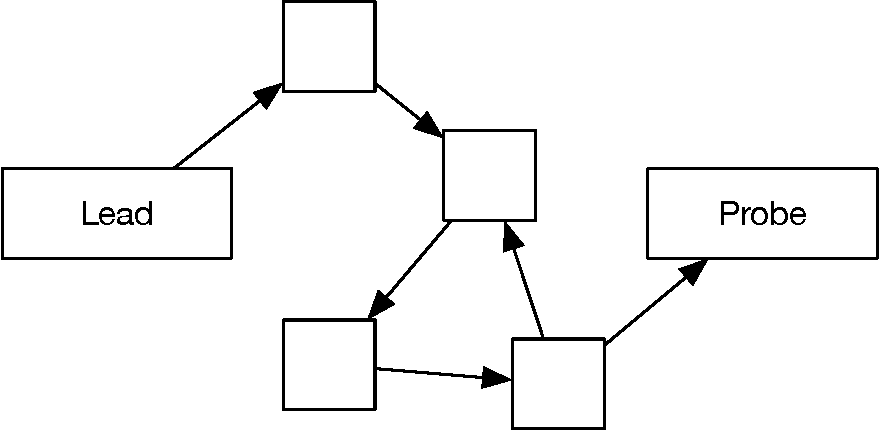
\includegraphics[width=2.5in]{LeadProbe.pdf}
\vspace{-1em}
\caption{A Lead and Probe at each end of a subgraph of Processes.}
\vspace{-1em}
\end{wrapfigure}

\subsection{Probe}

A Filter which gathers statistics on Resource flow.  A Probe can be used in two ways.  Either the Probe is used alone, in which case it measures the amount of Resource flowing through it; or the Probe can be used in conjunction with a {\bf Lead} to measure the statistics passing through a subgraph between them.   {\bf By default, this class's step() method does nothing, so there's no need to schedule it.}

Constructing a Probe is simple:

\begin{methods}{\class{sim.des.Probe} Constructor}
\mthd{public Probe(SimState state)}
Builds a Probe.  
\end{methods}

By itself, a Probe can be used to maintain statistics of data that flows through it:

\begin{methods}{\class{sim.des.Probe}}
\mthd{public void reset()}
Resets all statistics through the Probe.
\mthd{public double getSumThru()}
Returns the total amount of Resource passing through the Probe so far.
\mthd{public double getMaxThru()}
Returns the largest single amount of Resource passing through the Probe so far.
\mthd{public double getSumOffers()}
Returns the total number of offers passing through the Probe so far.
\mthd{public double getThruRate()}
Returns the average rate at which Resource is passing through the Probe so far.
\mthd{public double getOfferRate()}
Returns the average rate at which offers are made through the Probe so far.
\end{methods}

If you create a Lead, you can attach it at the start of a string of Processes, and the Probe at the end of the series, and together they will gather statistics on the information passing through the string.

\begin{methods}{\class{sim.des.Probe}}
\mthd{public Lead buildLead()}
Builds the Lead connected to this Probe.  At most one Lead can be connected to a Probe.
\mthd{public Lead getLead()}
Returns the Lead connected to this Probe, or null if one has not been built yet.
\end{methods}

With a Lead, the Probe can gather additional statistics:

\begin{methods}{\class{sim.des.Probe}}
\mthd{public double getRate()}
Returns average amount of Resource present in the string at any time.
\mthd{public double getIdleRate()}
Returns the average amount of time that the entire string is idle.
\mthd{public double getUtilizationRate()}
Returns the average amount of time that the entire string is operating (not idle).
\end{methods}


\subsection{Lead}

An object detached from Probe with can be used in combination with it to determine the amount of resources in a DES subgraph between them.   {\bf By default, this class's step() method does nothing, so there's no need to schedule it.}

\begin{methods}{\class{sim.des.Lead}}
\mthd{public Probe getProbe()}
Returns the Probe associated with this Lead.
\end{methods}


\section{Composed Processes}

\begin{wrapfigure}{r}{2.5in}
\vspace{-1em}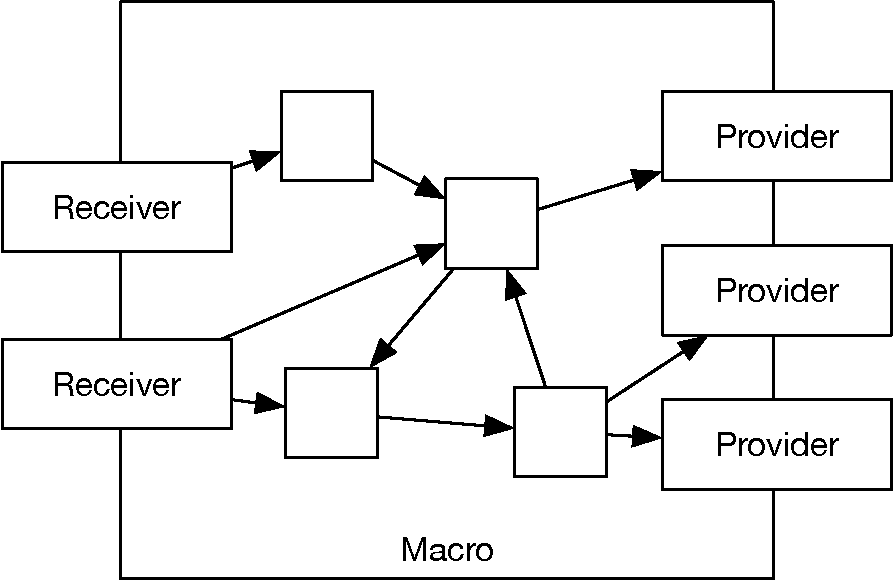
\includegraphics[width=2.5in]{Macro.pdf}
\vspace{-1em}
\caption{A Macro has some number of Receivers (which you provide) that are connected to a subgraph, and eventually output to some number of Providers (which you also provide).  The Receivers and Providers are connected to the outer world.}
\vspace{-2em}
\end{wrapfigure}

\subsection{Macro}

An object which can store a {\bf subgraph} of the DES graph.  This subgraph consists of some external-facing {\bf Receivers}, some external-facing {\bf Providers}, and some {\bf in-between Processes}.  When stepped, the Macro steps all of its stored objects in order.  You can access the Receivers and Providers external to the Macro to make offers or register stuff as you see fit.

The idea behind a Macro is that you can make a subclass of Macro which builds a custom subgraph, and then instantiate this Macro many times to recreate that subgraph in multiple locations.

Receivers are added with addReceiver(), Providers are added with addProvider(), and all other processes are added with add().  Macro is recursive: you can add Macros as part of the subgraph of other Macros (they are Parented like other process objects).

A Macro is the {\bf parent} of the Processes in its subgraph.  

\begin{methods}{\class{sim.des.Macro} Constructor}
\mthd{public Macro()}
Builds a Macro.  
\mthd{public Macro(String name)}
Builds a Macro with the given name.  
\end{methods}

\begin{methods}{\class{sim.des.Macro}}
\mthd{public boolean add(Parented obj, boolean step)}
Adds the object to the graph and indicates whether it should be stepped when Macro is stepped. 
\mthd{public boolean addReceiver(Receiver recv, boolean step)}
Adds the public (world-facing) receiver to the graph and indicates whether it should be stepped when Macro is stepped. 
\mthd{public boolean addProvider(Provider prov, boolean step)}
Adds the public (world-facing) provider to the graph and indicates whether it should be stepped when Macro is stepped. 
\mthd{public Receiver[] getReceivers()}
Returns all receivers.
\mthd{public String[] getReceiverNames()}
Returns the names of all receivers. 
\mthd{public Provider[] getProviders()}
Returns all providers.
\mthd{public String[] getProviderNames()}
Returns the names of all providers. 
\mthd{public void step(SimState state)}
Steps all registered objects in turn. 
\end{methods}

\subsection{Service}

\begin{wrapfigure}{r}{2.5in}
\vspace{-3em}
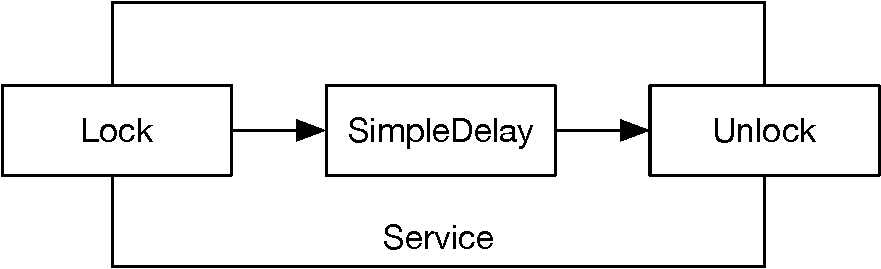
\includegraphics[width=2.5in]{Service.pdf}
\vspace{-1em}
\caption{A Service is a simple Macro with a Lock, a SimpleDelay, and an Unlock.}
\vspace{-7em}
\end{wrapfigure}

A simple example of a common Macro consisting of a Lock, then a SimpleDelay, then an Unlock.

\vspace{4em}

\begin{methods}{\class{sim.des.Service} Constructor}
\mthd{public Service(SimState state, Resource typical, Pool pool, double allocation, double delayTime)}
Creates a service with the given pool, allocation from the pool, and delay time.   

\mthd{public Service(SimState state, Resource typical, int initialResourceAllocation, double delayTime)}
Creates a service with a brand new private pool, initial resources in the pool, and delay time. Allocation is assumed to be 1.0
 \end{methods}

\begin{methods}{\class{sim.des.Service}}
\mthd{public Provider getProvider()}
Returns the provider (the Unlock).
\mthd{public Receiver getReceiver()}
Returns the receiver (the Lock).
\end{methods}



\bump

\begin{wrapfigure}{r}{2.5in}
\vspace{-1em}
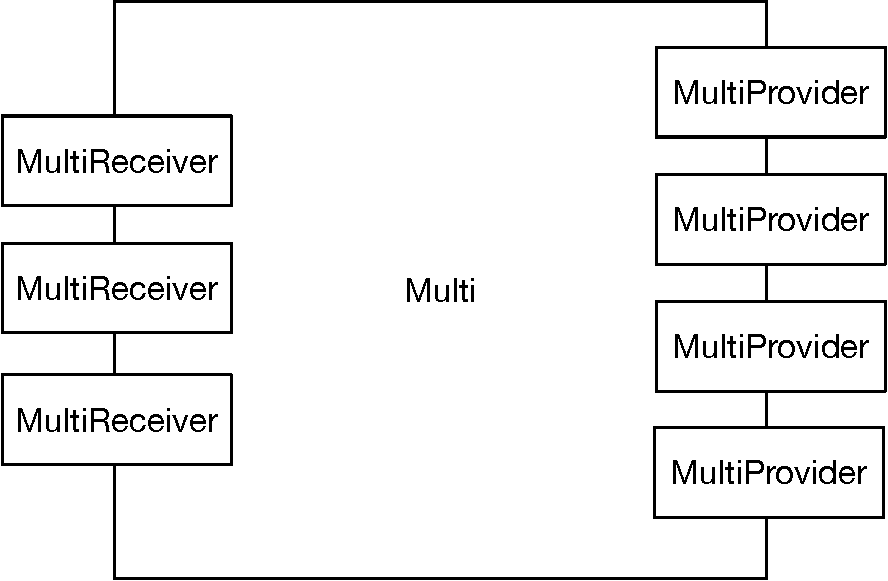
\includegraphics[width=2.5in]{Multi.pdf}
\vspace{-1em}
\caption{A Multi automatically sports some number of Receivers for different kinds of Resources, and some number of Providers for different kinds of Resources.  The Receivers and Providers are connected to the outer world.Offers or Provide requests to these Receivers or providers trigger method calls in the Multi which you can override. }
\end{wrapfigure}

\subsection{Multi}

An object which contains multiple Providers and multiple Receivers, all with potentially different typical Resource types, and so which can work with a variety of Resources simultaneously.    You do not provide the Providers or Receivers: instead you indicate an array of Resources for Providers and an array for Receivers, and the Multi will make its own custom Provider and Receiver subclasses, called {\bf MultiProviders} and {\bf MultiReceivers}, which communicate with the Multi when receiving resources or asked to provide resources.  You subclass from Multi to override the methods these custom Providers and Receivers will call, or to direct them to perform actions.

A Multi can also initiate transactions, and via a special Middleman called a {\bf Broker} it can be the recipient of a transaction.

You begin by constructing a Multi with the requested resources, and it builds the receivers and providers.  From there, you can access and manipulate these Receivers and Providers externally to communicate with the Multi.  You might want to register your Receivers as appropriate, and register other Receivers with your Providers.

\begin{methods}{\class{sim.des.Multi} Constructor}
\mthd{public Multi(SimState state, Resource[] receiverResources, Resource[] providerResources)}
Builds a Multi with a set of Receivers and a set of Providers, each with the following typical resources.
 \end{methods}

\begin{methods}{\class{sim.des.Multi}}
\mthd{public SimState getState()}
Returns the SimState.
\mthd{public int getNumReceivers()}
Returns the number of receivers.
\mthd{public int getNumProviders()}
Returns the number of providers.
\mthd{public Receiver[] getReceivers()}
Returns all receivers.
\mthd{public Provider[] getProviders()}
Returns all providers.
\mthd{public Receiver getReceiver(int receiverPort)}
Returns receiver \#receiverPort in the receivers array.
\mthd{public Provider getProvider(int providerPort)}
Returns provider \#providerPort in the providers array.
\mthd{public Receiver getReceiver(Resource resource)}
Returns the Multi Receiver meant to receive the following kind of resource, or null if there isn't one.  Note that if
		this Resource was given multiple times in the constructor, only the last Receiver is returned. 
		It's possible, indeed reasonable for you to have multiple receivers for a given resource for some
		modeling task: in this case, if the resource appeared in slots 5 and 7 (say) of the receiverResources[]
		array passed into the constructor, then the two corresponding receivers would be at ports 5 and 7. \mthd{public Provider getProvider(Resource resource)}
Returns the Multi Provider meant to receive the following kind of resource, or null if there isn't one.  Note that if
		this Resource was given multiple times in the constructor, only the last Provider is returned. 
		It's possible, indeed reasonable for you to have multiple providers for a given resource for some
		modeling task: in this case, if the resource appeared in slots 5 and 7 (say) of the providerResources[]
		array passed into the constructor, then the two corresponding Providers would be at ports 5 and 7.
\mthd{public String getName()}
Returns the Multi's name.
\mthd{public void setName(String name)}
Sets the Multi's name.
\mthd{public Object getParent()}
Returns the Multi's parent.
\mthd{public void setParent(Object parent)}
Sets the Multi's parent.
\end{methods}

\paragraph{MultiReceivers and MultiProviders}
When a MultiReceiver or MultiProvider is accessed, it will call a method on the Multi.  You can override this method to process the request.

\begin{methods}{\class{sim.des.Multi}}
\mthd{protected boolean accept(int receiverPort, Provider provider, Resource resource, double atLeast, double atMost)}
Called when a Multi receiver receives an offer.  The receiver in question is specified by its receiverPort. 
        Override this to process offers, in the same way that a Receiver processes an offer via its accept(...) method.  
        By default this method returns false.  
\mthd{protected boolean provide(int providerPort, Receiver receiver, Resource resource, double atMost)}
Called when a Multi provider receives a request to make an offer.  The provider in question is specified by its providerPort. 
        Override this to make an offer if you see fit by calling provide(...).  By default this method returns false.  
\end{methods}
 
From within your Multi, you can then make provide requests or make offers through the MultiReceivers or MultiProviders.  As usual, the Multi checks for cycles via isOffering().
 
\begin{methods}{\class{sim.des.Multi}}
\mthd{protected boolean requestProvide(int receiverPort, Provider provider, double atMost)}
Instructs a Multi receiver to ask some provider to make an offer by calling its provide(..., atMost) method.
        The receiver in question is specified by its receiverPort. 
\mthd{protected boolean requestProvide(int receiverPort, Provider provider)}
Instructs a Multi receiver to ask some provider to make an offer by calling its provide(...) method.
        The receiver in question is specified by its receiverPort. 
\mthd{protected boolean offerReceivers(int providerPort, Resource resource, double atLeast, double atMost)}
Instructs a Multi provider to make an offer by calling offerReceivers(...) method, and then
        offer the resource as specified. 
\mthd{protected boolean isOffering()}
Returns true if the Provider is currently making an offer to a receiver (this is meant to allow you
        to check for offer cycles. 
 \mthd{public void reset(SimState state)}
By default does nothing
\mthd{public void step(SimState state)}
By default does nothing.
\end{methods}
 
 \paragraph{Transactions}
 
Like Middleman, Multi can also perform transactions.  To initiate a transaction with a Middleman, you can call offerTransaction(...).  You can also create a {\bf broker}, essentially a custom Middleman, which is connected to one MultiReceiver and one MultiProvider.  This broker can receive transaction requests from external Middlemen.  On transaction request, the Broker then calls performTransaction() on the Multi, which you may override as you see fit to process the transaction.
 
\begin{methods}{\class{sim.des.Multi}}
\mthd{protected Resource offerTransaction(int providerPort, int receiverPort, Middleman middleman, Resource provided,}
\rule{0pt}{0pt}\hspace{\fill}{\sf double atLeast, double atMost, Resource requestedType, double atLeastRequested)}\\
Instructs a Multi to offer a transaction to a Middleman, notionally from the Multi's provider and receiver ports,
    	though they really won't come into it. If the transaction is agreed to, your provided resource will be accordingly 
    	modified (reduced) and the requested resource will have been provided.  Otherwise null will be returned.
		
The transaction is offering atLeast and atMost a certain amount of provided resource in exchange for
    	(from you) a requested resource.  atLeastRequested is the amount of requested resource to be provided
    	in exchange for the *least* amount of provided resource.  If you decide to take some X provided resource
    	where X is between atLeast and atMost, then the resource amount you provide in return is 
	\code{X * atLeastRequested / atMost}.
    	For requested CountableResources, I suggest that the amount returned in response to a request would best be
    	\code{(int)(X * atLeastRequested / atMost)}, but you can do as your model deems appropriate.
    	
For Entities, only a single Entity can be provided.  If an Entity is being provided, then atLeast = atMost = 1.
    	
For Entities, only a single Entity can be requested.  If an Entity is being requested, atLeastRequested = 1
    	and exactly one Entity should be returned regardless of its value, and atLeast = atMost. 
    	
Don't override this method.  Instead, override performTransaction().

\mthd{public Middleman getBroker(final int providerPort, final int receiverPort)}
Builds a Middleman from the given provider and receiver ports solely for the purpose of performing a transaction.
    	This is thus a "Broker", a simplified Middleman which refuses offers and requests to make offers: it only responds
    	to requests to make transactions, that is, transact(...).  Note that if you call this method twice with the
    	same provider and receiver ports, you will receive different Middlemen.
    	
This Middleman will refuse a transaction if the Receiver associated with the underlying receiver port
    	is set to refuse offers. 
    	
Also note that the Multi has a global check for zero-time transaction cycles going 
    	through it.  That is, you can't make a transaction through one provider/receiver port pair, and have it make
    	its way through a chain of zero-time transactions to wind up trying to transact through a second
    	provider/receiver port pair on the same Multi. 
	
\mthd{protected Resource performTransaction(int myProviderPort, int myReceiverPort, Provider provider, Receiver receiver,}
\rule{0pt}{0pt}\hspace{\fill}{\sf Resource provided, double atLeast, double atMost, Resource requestedType,}\\ \rule{0pt}{0pt}\hspace{\fill}{\sf double atLeastRequested)}\\
Received by the Multi when an external Provider and Receiver are asking for a transaction of one resource for another,
    	by building a Middleman to broker with a provider port and receiver port on the Multi, though the ports really won't
    	come into it.  
    	The Provider would provide a resource to the Multi and a Receiver would receive the transacted returned Resource.
    	Very commonly this Provider and Receiver are one and the same: they are a Middleman or perhaps a Multi. 
    	But this does not have to be the case.  	
		If the transaction is agreed to, you should modify the provided resource and return the requested resource.
		Otherwise, return null.  The default form simply returns null. 
		
By the time this method has been called, refuses-offers,
		cyclic, and type compatibility checks have already been performed, but you might still benefit from 
		knowing the requestedType, so it is provided: but you should not modify this resource nor return it.
				
The transaction is offering atLeast and atMost a certain amount of provided resource in exchange for
    	(from you) a requested resource.  atLeastRequested is the amount of requested resource to be provided
    	in exchange for the *least* amount of provided resource.  If you decide to take some X provided resource
    	where X is between atLeast and atMost, then the resource amount you provide in return 
	\code{X * atLeastRequested / atMost}.
    	For requested CountableResources, I suggest that the amount returned in response to a request would best be
    	\code{(int)(X * atLeastRequested / atMost)}, but you can do as your model deems appropriate.
    	
For Entities, only a single Entity can be provided.  If an Entity is being provided, then atLeast = atMost = 1.
    	
For Entities, only a single Entity can be requested.  If an Entity is being requested, atLeastRequested = 1
    	and exactly one Entity should be returned regardless of its value. 
\end{methods}

\begin{wrapfigure}{r}{3.5in}
\vspace{-3em}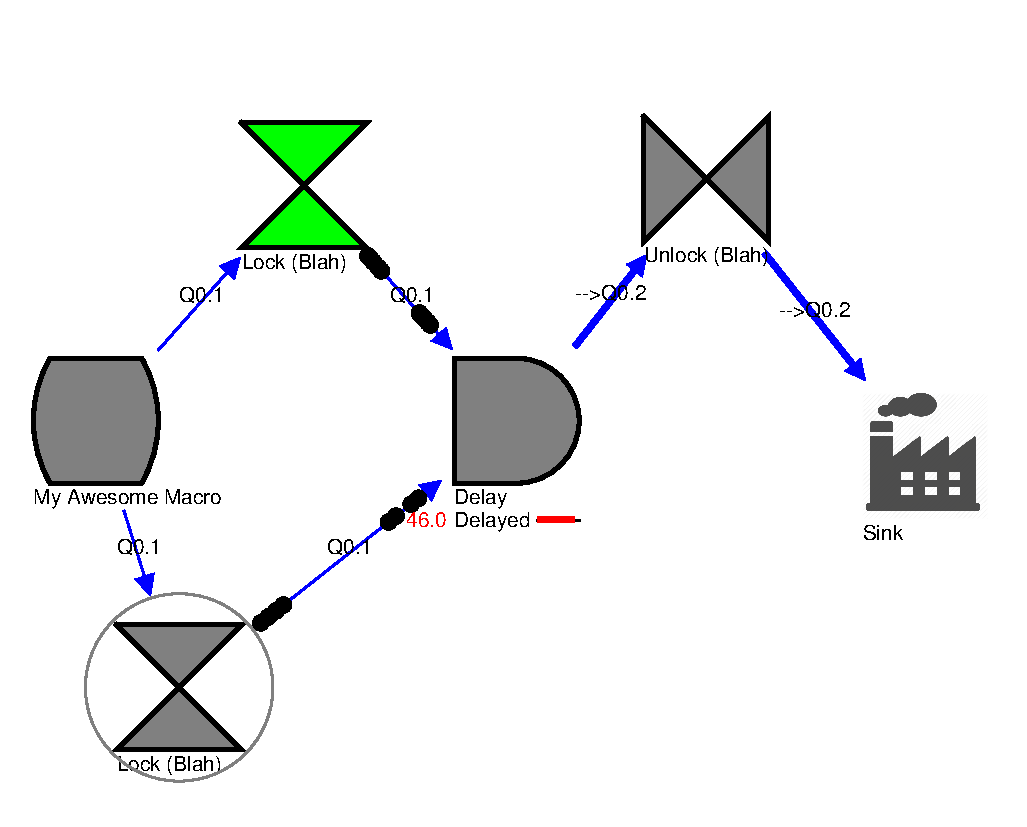
\includegraphics[width=3.5in]{Visualization.pdf}
\vspace{-2em}
\caption{Visualization Example.  This shows processes of different shapes, plus a Macro.  The Sink object is displayed with an image rather than a shape.  One Lock is being displayed with a different fill color.  The other Lock is currently circled, indicating that it's in a locked state.  The Delay is shown with a bar indicating the amount delayed.  Edges entering the Delay are DelayPortrayals, showing the delayed elements and how long each has before it is no longer delayed.  The remaining edges are ResourceEdgePortrayals, with different thicknesses indicating amount of Resource traveling along them.  Edges are labeled in the form ``Q{\it value}''.  Q stands for ``Quatloos'', a type of money (the Resource being transferred), and the value is the last amount offered.  A little arrow next to the ``Q'' indicates that the Resource is being transferred right now.}
\label{visualization}
\end{wrapfigure}

\section{Visualization and Statistics}

MASON at present has relatively rudimentary display options for its DES toolkit.  With time I expect this to improve.

DES objects are visualized (in 2D) exactly in the same way that standard MASON objects are visualized: a {\bf Display2D} holds one or more {\bf Field Portrayals} (in this case, a {\bf Continuous2DPortrayal} to visualize the process objects overlaid with a {\bf NetworkPortrayal} to visualize their connections).  

Beyond this it gets specialized.  In the DES system, the NetworkPortrayal holds not a SpatialNetwork2D to tell it the objects and their edges, but a {\bf DES2D}, which is designed to make it easy to build the graph structure: just add the processes and state their connections, or let it figure out the connections on its own.   

Inside a DES2D, each DES Provider, Sink, Macro, Multi, and Pool are all subclasses of {\bf DESPortrayal}, a special SimplePortrayal2D which draws these objects with special shapes, images, and/or colors.    DESPortrayal is an {\bf InternalPortrayal2D} because it actually uses a {\bf ShapePortrayal2D} or {\bf ImagePortrayal2D} to do the actual drawing, InternalPortrayal2D helps it get around the fact that these portrayals are not java.io.Serializable.  The class {\bf DESPortrayalParameters} holds overall parameters regarding the global scaling of these portrayals.  These objects also have one or more labels via a {\bf LabelledPortrayal2D} to describe features of the objects.  Some objects also can provide small bar charts alongside their labels, using a special subclass called {\bf BarPortrayal}.

Connections among the objects are handled in the DES2D using an internal object called a {\bf ResourceEdge} (along which Resources may flow).  There are two kinds of EdgePortrayals available for ResourceEdge.  A {\bf ResourceEdgePortrayal} changes its thickness as more resources flow along it.  And a {\bf DelayedEdgePortrayal}, when connected to a SimpleDelay, Delay, or BoundedDelay, shows delayed resources as if they were traveling along the edge.

Macros have their own cute feature.  If you triple-click on a Macro's portrayal, it will open up a new Display showing the contents of the Macro.  Note that only the Macro subgraph is shown, not Providers or Receivers connected to it.  That might be a bit confusing.


\begin{figure}[t]
\centering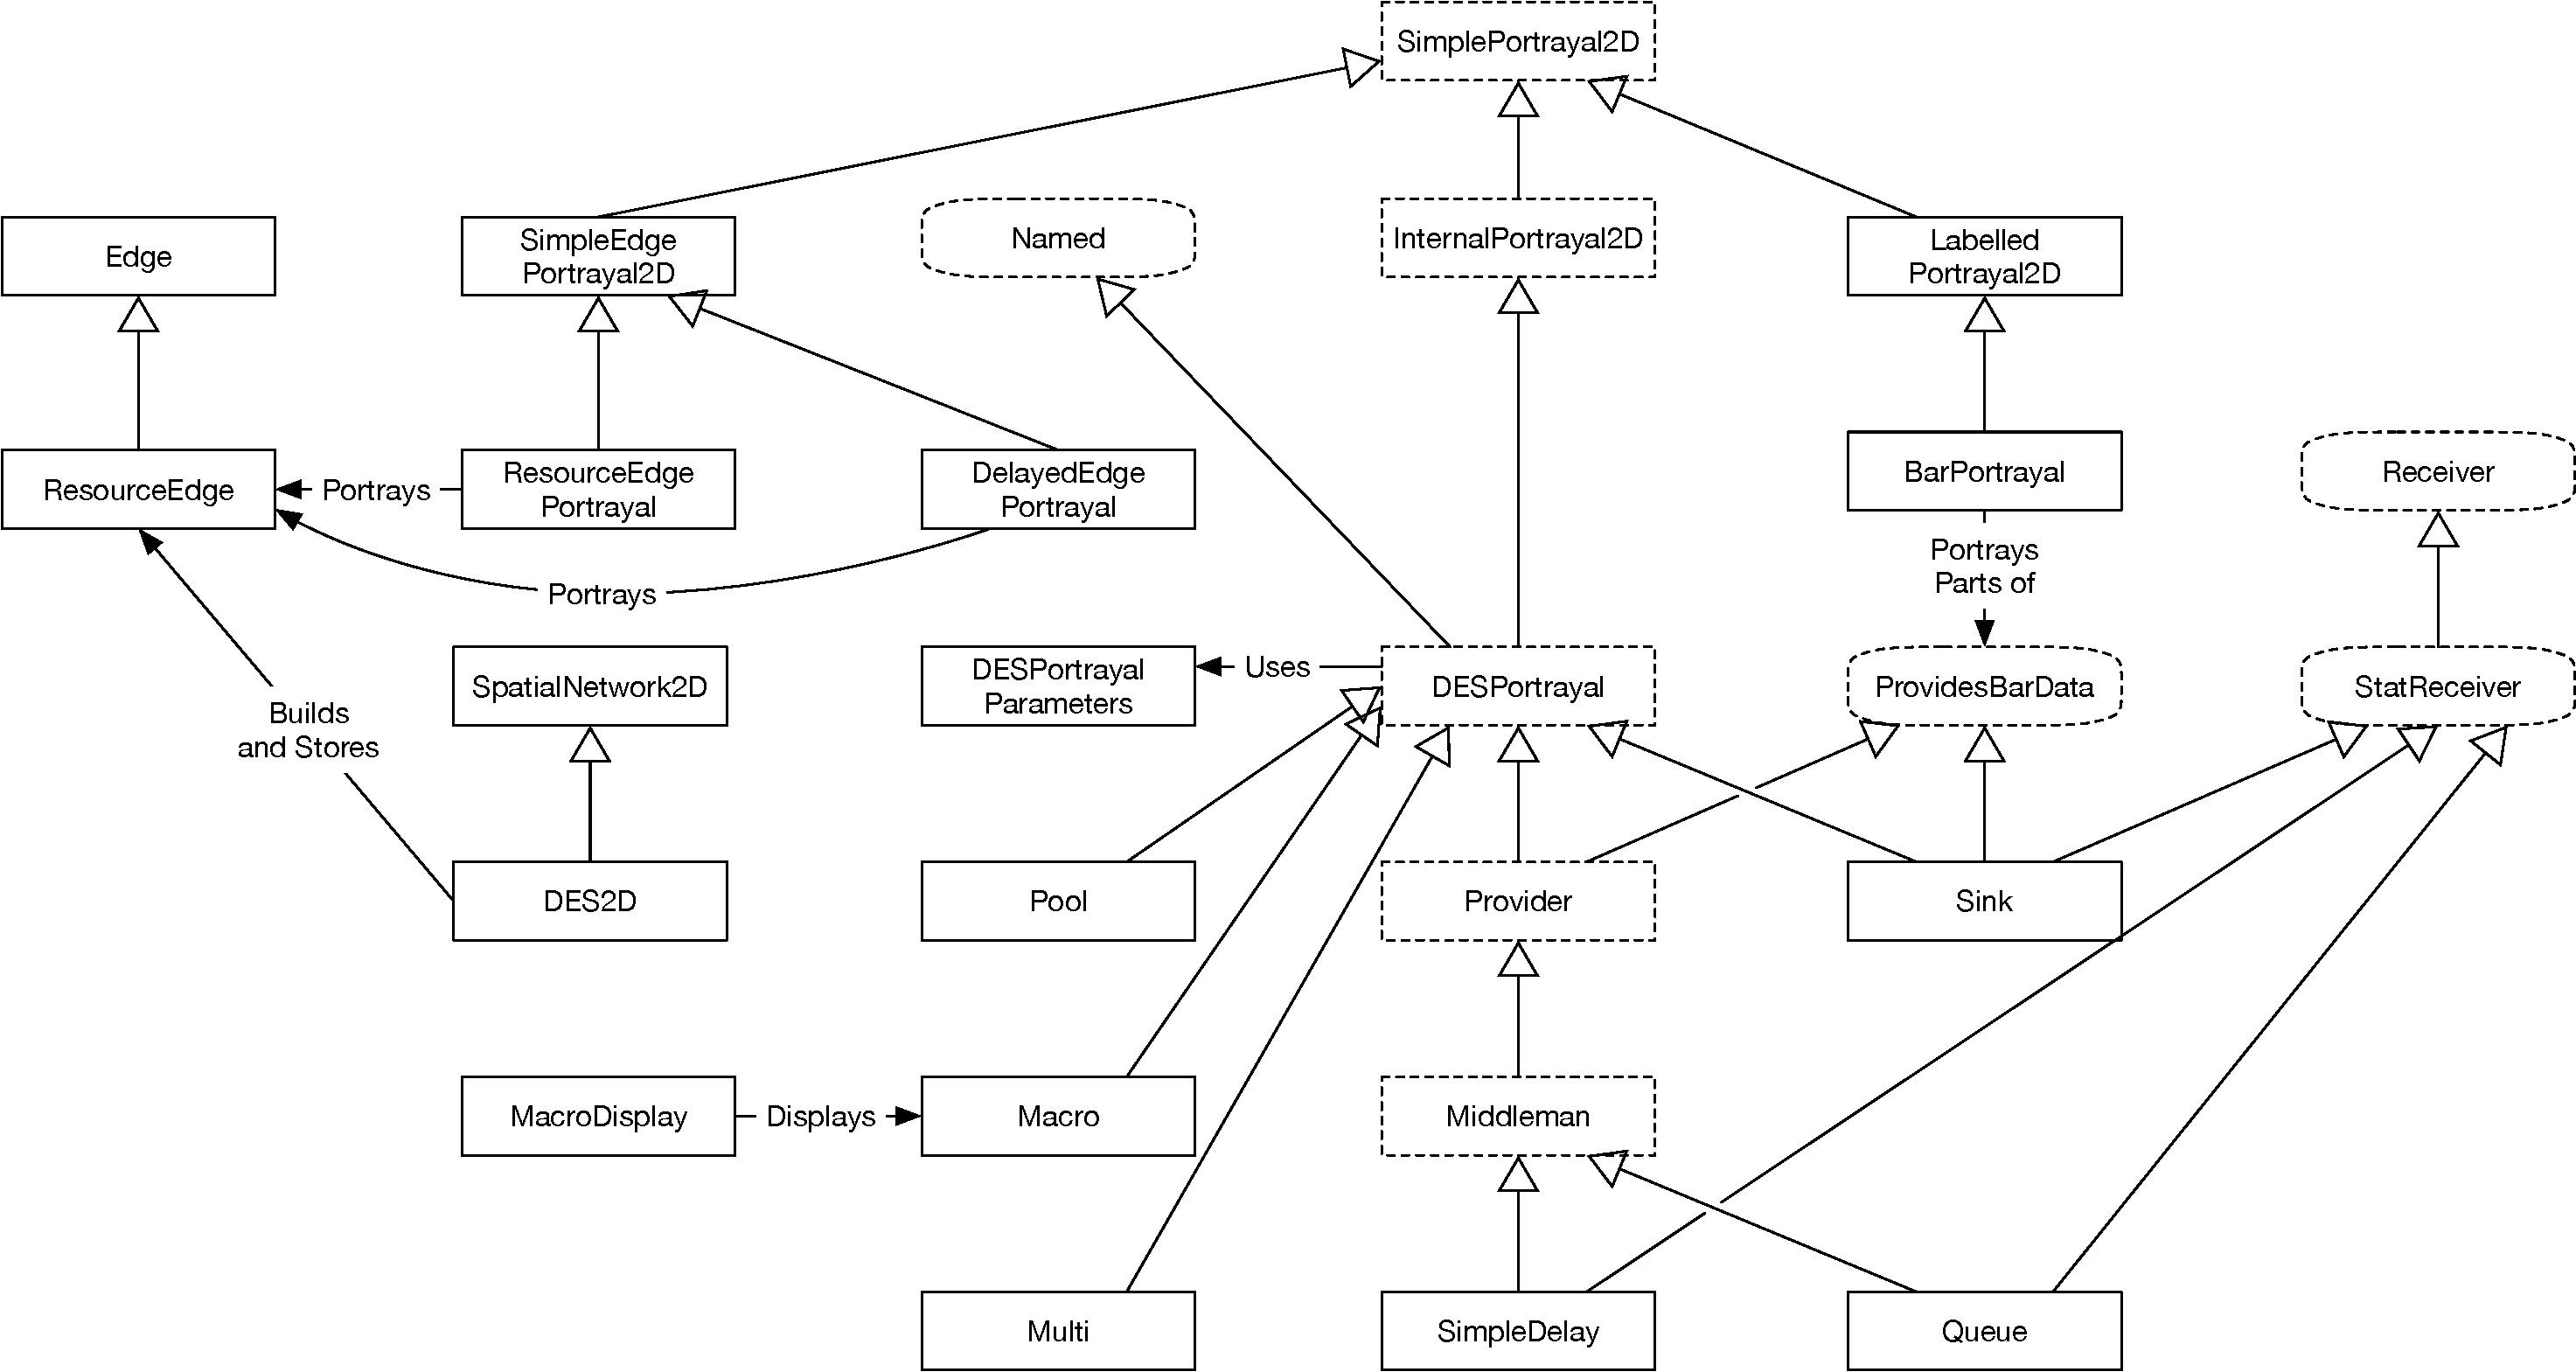
\includegraphics[width=6.5in]{VisualizationUML.pdf}
\caption{Visualization facility, with only primary object relationships shown.}
\end{figure}


\subsection{DESPortrayal}

All processes, along with Multis, Pools, and Macros, are all subclasses of DESPortrayal, so they can portray themselves easily.  As you can see in Figure~\ref{visualization}, these objects can be portrayed with a variety of shapes (each object class has a different default shape), with custom images, and with custom colors.  The processes can also be accompanied by a number of labels underneath providing additional information, and Locks can be circled, indicating whether the Lock is, well, locked.

In order to portray itself properly, all a DESPortrayal subclass needs to do is override the method \method{buildDefaultPortrayal(double scale)} to return an appropriate SimplePortrayal using the current fill, stroke, stroke width, and scale.  

For example, SimpleDelay does this:

\begin{verbatim}
    public SimplePortrayal2D buildDefaultPortrayal(double scale)
        {
        return new ShapePortrayal2D(ShapePortrayal2D.SHAPE_DELAY, 
            getFillPaint(), getStrokePaint(), getStrokeWidth(), scale);
         }
\end{verbatim}

This can be overridden when you instantiate a DES object in your model, such as:

\begin{verbatim}
    SimpleDelay simple = new SimpleDelay(...)
        {
        SimplePortrayal2D buildDefaultPortrayal(double scale)
                {
                new ShapePortrayal2D(ShapePortrayal2D.POLY_SQUARE,
                        Color.BLUE, Color.RED, 2.0, scale);
                 }
         };
\end{verbatim}

You can change the fill color by calling \method{setFillPaint(...)} on the SimpleDelay object; and similarly the stroke paint and stroke width.  This can be done dynamically as well, in the middle of your model.

You can also entirely replace the shape with an image.  This is very simple, you just set the image by calling the method \method{setImage(...)} and the default shape portrayal will be replaced.  You could do this in the object's constructor, or you could do it when instantiating the object in the model, such as:

\begin{verbatim}
    simple.setImage("images/factory.png", true);
\end{verbatim}

This means to look for the \file{factory.png} file in a directory called \file{images} located right next to the class file of the {\bf image class} specified in DESPortrayalParameters.  By default this is DESPortrayalParameters.class, which isn't very helpful.  In your GUIState's \method{init(...)} method, you should set this to something more useful, such as:

\begin{verbatim}
    DESPortrayalParameters.setImageClass(MyDESExampleWithUI.class);
\end{verbatim}

Now, the \file{images} directory will be located next to your MyDESExampleWithUI.class file.  Alternatively if you said 

\begin{verbatim}
    simple.setImage("images/factory.png", false);
\end{verbatim}

... then MASON would look for the \file{images} directory relative to the SimpleDelay.class file.  This isn't very useful, but if you {\it subclassed} this the SimpleDelay class, perhaps making an anonymous subclass, then it'd look for the directory relative to that subclass.

\begin{methods}{\class{sim.des.portrayal.DESPortrayal}}
\mthd{public Paint getFillPaint()}
Returns the fill paint for the underlying default portrayal shape. 
\mthd{public void setFillPaint(Paint paint)}
Sets the fill paint for the underlying default portrayal shape.  Note that calling this method will fire up Java's GUI subsystem.   
\mthd{public Paint getStrokePaint() }
Returns the stroke paint for the underlying default portrayal shape. 
\mthd{public void setStrokePaint(Paint paint) }
Sets the stroke paint for the underlying default portrayal shape.  Note that calling this method will fire up Java's GUI subsystem.  
\mthd{public double getStrokeWidth() }
Returns the stroke width for the underlying default portrayal shape. 
\mthd{public void setStrokeWidth(double width) }
Sets the stroke width for the underlying default portrayal shape. 
\mthd{public void setImage(String path, boolean usesGlobalImageClass)}
Sets the path to the image file, relative to the class file in setImageClass(). 
\mthd{public String getImagePath()}
Returns the path to the image file, relative to the class file in setImageClass(). 
\mthd{public boolean getUsesGlobalImageClass() }
Returns the class file from which setImagePath(...) defines a path to the image, if any. 

\mthd{public boolean getDrawState() }
Indicates if the portrayal should currently be drawn circled.  Some subclasses, such as Lock,
        may change this value in real time. 
\mthd{public SimplePortrayal2D providePortrayal(Object object)}
Called by InternalPortrayal2D to provide the portrayal to draw this object.
        We override the standard method to update the scale and rebuild the portrayal
        if the scale is wrong.  Don't play with this.
\mthd{public SimplePortrayal2D buildPortrayal(Object object)}
        Called by InternalPortrayal2D to build a new portrayal when called for.
        To do this, it first either builds an ImagePortrayal2D (if you have set the baseImagePath),
        or a ShapePortrayal2D of some sort (returned by buildDefaultPortrayal(....)). 
        It then attaches to this base portrayal a variety of labels, indicators, and the ability
        to move.  The final modified portrayal is then returned.  You probably shouldn't play with this.
\mthd{public SimplePortrayal2D buildDefaultPortrayal(double scale)}
        Builds the "base portrayal" for the object, if the image path and class haven't been set (and thus
        the portrayal isn't an ImagePortrayal2D).  The default sets to a simple gray and black quare.
\mthd{public ImagePortrayal2D buildDefaultImagePortrayal(ImageIcon icon, double scale)}
        Builds an "image portrayal" for the object, if the image path and class have been set.  
    	Normally you'd not bother overriding this method (though Macro does to customize its triple-clicking
    	feature). The default just makes a basic ImagePortrayal2D.  Don't override this unless you need a 
	custom way of loading and building an ImagePortrayal2D.
\end{methods}



\subsection{DESPortrayalParameters}

This class stores global parameters which affect all the DES portrayals together, notably their default scaling and image classes.



\begin{methods}{\class{sim.des.portrayal.DESPortrayalParameters}}
\mthd{public static double getPortrayalScale() }
Returns the scaling for DESPortrayals.  By default this is 10.0.
\mthd{public static void setPortrayalScale(double scale) }
Sets the scaling for DESPortrayals.  By default this is 10.0.
\mthd{public static void setImageClass(Class cls) }
Sets the class whose class file location is where we'll start the image path to load images.  By default this is DESPortrayalParameters.class, not very useful.
\mthd{public static Class getImageClass() }
Returns the class whose class file location is where we'll start the image path to load images.
\end{methods}

\subsection{ProvidesBarData}

Some DESPortrayals provide small bar charts with labelled data below their primary label.  To do this, they implement ProvidesBarData.  This interface contains three public variables:

\begin{verbatim}
    public double[] getDataBars();
    public String[] getDataValues();
    public String[] getDataLabels();
\end{verbatim}

These arrays must be the same length, and each slot represents a separate labeled line.  \variable{getDataBars()[i]} holds the size of the data bar for line {\it i}, from 0 to 1 inclusive.  If it is -1 then there is no data bar.  \variable{getDataValues()[i]} holds the string value corresponding to the size.  \variable{getDataLabels()[i]} holds the label of the data element.  You can have as many lines as you like.  See SimpleDelay for an example of usage.  You can see examples of objects with bars in Figure~\ref{visualization}, page~\pageref{visualization}.

\subsection{BarPortrayal}

BarPortrayal is the Wrapper Portrayal which provides bar data display.  It's just a subclass of LabelledPortrayal2D.  You normally don't work with this class, as it's handled internally by DESPortrayal.   You can see examples of objects with bars in Figure~\ref{visualization}, page~\pageref{visualization}.

\subsection{DES2D}

DES2D is designed to make it easy to create and display a DES model graph.  You just create a DES2D, then add objects one by one, along with their locations in space.  You can connect them manually, or you can just connect them all automatically at the end with a single method call.  The DES2D object is then used by your NetworkFieldPortrayal2D and ContinuousPortrayal2D to portray the objects.  See \file{sim/app/desexample/} for an example of how to use this in a standard MASON structure.

What I'd do is:

\begin{enumerate}
\item Use \method{add(...)} to add every object (Provider, Receiver, Multi, Macro, and Pool if you want to) in the DES graph.
\item Use \method{connectAll()} to connect everything
\end{enumerate}

... and you're done.

\begin{methods}{\class{sim.des.portrayal.DES2D} Constructor}
\mthd{public DES2D(double width, double height)}
Builds a DES2D with the given region.
\end{methods}

\begin{methods}{\class{sim.des.portrayal.DES2D}}
\mthd{public void add(Object obj, Double2D location)}
Adds the given object at the provided location.
\mthd{public void add(Object obj, double x, double y)}
Adds the given object at the provided location.
\mthd{public ResourceEdge connect(Provider provider, Receiver receiver)}
Connects a provider to a receiver.  You ought to have added them first.
\mthd{public ResourceEdge connect(Provider provider, Receiver receiver, Object in)}
Connects a provider to a receiver stored in the Macro ``in''.  
The edge will go from the provider to the ``in'' Macro; but its thickness and other state features
will be determined not by querying the ``in'' Macro but by querying the receiver.  
This is often used for Macros: you'd set ``in'' to a Macro, and receiver to the actual Receiver in the Macro
that the Provider is communicating with.  You ought to have added provider and in.
\mthd{public ResourceEdge connect(Macro out, Provider provider, Receiver receiver)}
Connects a provider stored in the Macro ``out'' to a receiver.  
The edge will go from the ``out'' Macro to the receiver; but its thickness and other state features
will be determined not by querying the ``in'' Macro but by querying the provider.  
This is often used for Macros: you'd set ``out'' to a Macro, and provider to the actual Provider in the Macro
that the Receiver is communicating with.  You ought to have added receiver and out.
\mthd{public ResourceEdge connect(Macro out, Provider provider, Receiver receiver, Object in)}
Connects some Macro ``out'' to another Macro ``in'' using their respective providers and receivers.
The edge will go from the ``out'' Macro to the ``in'' Macro; but its thickness and other state features
will be determined not by querying the ``in'' and ``out'' Macros but by querying the provider and receiver.  
This is often used for Macros: you'd set ``in'' and ``out'' to Macros, and provider and receiver to the 
actual Provider and Receiver in the Macros that are communicating.  You ought to have added in and out.
\mthd{public ResourceEdge connect(Multi out, int portOut, Receiver receiver)}
Connects a Multi with a given output Provider to  the given receiver.
\mthd{public ResourceEdge connect(Provider provider, Multi in, int portIn)}
Connects a Multi with a given input Receiver to  the given Provider.
\mthd{public ResourceEdge connect(Multi out, int portOut, Receiver receiver, Object in)}
Connects a Multi with a Macro with the given receiver.
The edge will go from the Multi to the ``in'' Macro; but its thickness and other state features
will be determined not by querying the ``in'' Macro but by querying the receiver.  
 You ought to have added out and in.
\mthd{public ResourceEdge connect(Multi out, Provider multiProvider, Receiver receiver, Object in)}
Connects a Multi's provider with a Macro with the given receiver.
The edge will go from the Multi's provider to the ``in'' Macro; but its thickness and other state features
will be determined not by querying the ``in'' Macro but by querying the receiver and provider
 You ought to have added out and in.
\mthd{public ResourceEdge connect(Object out, Provider provider, Multi in, int portIn)}
Connects some Macro ``out'', with its provider, to a Multi ``in'' with the given input port receiver.
The edge will go from the ``out'' Macro to the ``in'' Multi; but its thickness and other state features
will be determined not by querying the ``in'' and ``out'' Macro/Multi objects but by querying the provider and receiver.  
You ought to have added in and out.
\mthd{public ResourceEdge connect(Multi out, int portOut, Multi in, int portIn)}
Connects some Multi ``out'' to a Multi ``in'' with the given input port receiver and output port providers.
The edge will go from the ``out'' Multi to the ``in'' Multi; but its thickness and other state features
will be determined not by querying the ``in'' and ``out'' Multi objects but by querying their provider and receiver.  
You ought to have added in and out.
\mthd{public ArrayList\(<\)ResourceEdge\(>\) connect(Provider provider)}
Make all the outgoing connections for the given Provider.  The Provider and all of its Receivers should have been added.
\mthd{public ArrayList\(<\)ResourceEdge\(>\) connect(Multi multiProvider)}
Make all the outgoing connections for the given Multi.  The Multi and all of the Receivers connected to its Providers should have been added.
\mthd{public ArrayList\(<\)ResourceEdge\(>\) connect(Macro macroProvider)}
Make all the outgoing connections for the given Macro.  The Macro and all of the Receivers connected to its Providers should have been added.
\mthd{public ArrayList\(<\)ResourceEdge\(>\) connectAll()}
Make all connections for any objects added so far.
\mthd{public void clear()}
Remove all objects and connections.
\mthd{public Continuous2D getNodes()}
Return the network Nodes (used in NetworkPortrayal2D).
\mthd{public Network getEdges()}
Return the network edges (used in NetworkPortrayal2D).
\end{methods}

\subsection{ResourceEdge}

ResourceEdge is the edge type used in DES2D to connect objects.  It's a subclass of Edge.  You don't need to know much about it except to understand that it has four connections:

\begin{itemize}
\item FROM is the object the edge leaves from (when drawn)
\item TO is the object the edge goes to (when drawn)
\item PROVIDER is the provider of resources along the edge
\item RECEIVER is the receiver of resources along the edge
\end{itemize}

Why are TO and PROVIDER distinct, and why are FROM and RECEIVER distinct?  This is for Macros and Multis.  You might want an edge from (say) a SimpleDelay to a receiver in a Multi: but you're not drawing the receiver, you're only drawing the Multi as a single object.  However you want the edge to change in thickness etc. in response to the receiver (not the Multi).  Thus the Multi is TO but its receiver is RECEIVER.  See DES2D, which distinguishes these in its Macro and Multi methods

Like all Edges, ResourceEdge has an Info (label) object returned by getInfo(). By default, this object is a string indicating the current resource being provided along the edge.

\subsection{ResourceEdgePortrayal}

This is a special subclass of EdgePortrayal which you can use to portray the connections between objects in your GUIState.  It behaves just like EdgePortrayal, except that it adjusts its thickness according to the amount of Resource presently being provided along the edge.  Additionally, you can customize the paint of the edge on a per-resource type basis.  You can see examples of ResourceEdgePortrayal in Figure~\ref{visualization}, page~\pageref{visualization}.

\begin{methods}{\class{sim.des.portrayal.ResourceEdgePortrayal} Constructor}
\mthd{public ResourceEdgePortrayal()}
Builds a ResourceEdgePortrayal with a default scale of 1.0, and using a standard line.

\mthd{public ResourceEdgePortrayal(boolean triangle)}
Builds a ResourceEdgePortrayal with a default scale of 1.0, and using either a triangle or standard line.

\mthd{public ResourceEdgePortrayal(double scale)}
Builds a ResourceEdgePortrayal with the given default scale, and using a standard line.

\mthd{public ResourceEdgePortrayal(double scale, boolean triangle)}
Builds a ResourceEdgePortrayal with the given default scale, and using either a triangle or standard line.
\end{methods}

\begin{methods}{\class{sim.des.portrayal.ResourceEdgePortrayal}}
\mthd{public void putPaint(int resourceType, Paint paint)}
Paint the edge the given paint when it transfers the given resource type.

\mthd{public Paint getPaint(int resourceType)}
Return the paint used for the given resource type.
\mthd{protected double getPositiveWeight(Object edge, EdgeDrawInfo2D info)}
Return the (positive) weight for the edge to change its thickness.  By default this returns a weight according to the received amount, scaled by the given edge scale.
\end{methods}

\subsection{DelayedEdgePortrayal}

This is a special subclass of EdgePortrayal designed to be connected to the {\it input} (Receiver end) of SimpleDelay, Delay, and BoundedDelay.  It queries these delays for their current delayed objects arriving from the corresponding Provider, and draws the objects along the edge to show them ``arriving'' to the delay.  You can see examples of DelayedEdgePortrayal in Figure~\ref{visualization}, page~\pageref{visualization}.

\begin{methods}{\class{sim.des.portrayal.ResourceEdgePortrayal}}
\mthd{public void putPaint(int resourceType, Paint paint)}
Paint the edge the given paint when it transfers the given resource type.
\mthd{public Paint getPaint(int resourceType)}
Return the paint used for the given resource type.
\mthd{public void putCirclePaint(int resourceType, Paint paint)}
Paint the markers (traveling along the edge) with the given paint when they have the given resource type.
\mthd{public Paint getCirclePaint(int resourceType)}
Return the paint used for the markers indicating for the given resource type traveling along the edge.
\mthd{protected double getPositiveWeight(Object edge, EdgeDrawInfo2D info)}
Return the (positive) weight for the edge to change its thickness.  By default this returns a weight according to the received amount, scaled by the given edge scale.
\end{methods}


\subsection{MacroDisplay}

A convenience class to create a new Display when the user triple-clicks on a Macro.  To do this, in GUIState.init(...) you create some \(N\) MacroDisplays, one for each Macro instance in your model.  Then in GUIState.setupPortrayals() (that is, in start() or load(...)) you attach a Macro to each MacroDisplay.  See \file{sim/app/desexample/} for an example.


\begin{methods}{\class{sim.des.portrayal.MacroDisplay} Constructor}
\mthd{public MacroDisplay(GUIState state, int width, int height, int macroNum)}
Create a MacroDisplay with the given GUIState, width, and height.  The macroNum is a unique number, displayed in the Display titlebar, to distinguish them from one another if you are displaying them prior to running the model.
\end{methods}

\begin{methods}{\class{sim.des.portrayal.MacroDisplay}}
\mthd{public void attachMacro(Macro macro, SimpleEdgePortrayal2D portrayal)}
Attach a MacroDisplay to given Macro.  The portrayal is used to specify the portrayal for all the edges in the MacroDisplay.  (We'll have to improve that later).
\end{methods}


%\cleardoublepage
%\footnotesize
%\addcontentsline{toc}{chapter}{Index}
%\printindex

\end{document}














